% =====================================================================
% Lyrebird — arXiv manuscript
% Rewritten from scratch, 2026-08-01, replacing docs/whitepaper/build_whitepaper.py
%
% NOTE TO THE AUTHOR — BIBLIOGRAPHY RECONCILIATION
% ------------------------------------------------------------
% docs/whitepaper/references/references.bib did not exist when this file was
% written. What exists is docs/whitepaper/references/REFERENCES.md — a verified
% ledger of 104 keyed entries (40 VERIFIED / 59 CORRECTED / 2 UNVERIFIABLE) with
% 57 PDFs in references/pdf/. The keys used here have been RENAMED to match that
% ledger. 63 of the 75 keys used are in it; the 12 that are not must be added,
% because they are methods and literature this manuscript cites that the
% repository never cited, so the ledger's audit did not cover them.
%
% MUST BE ADDED TO THE .bib (verified externally; not in REFERENCES.md)
%   beans2022      Hagiwara, Hoffman, Liu, Cusimano, Effenberger, Zacarian.
%                  BEANS: The Benchmark of Animal Sounds. ICASSP 2023, 1-5.
%                  doi 10.1109/ICASSP49357.2023.10096686
%   berwick2011    Berwick, Okanoya, Beckers, Bolhuis. Songs to syntax: the
%                  linguistics of birdsong. TiCS 15(3):113-121.
%                  doi 10.1016/j.tics.2011.01.002
%   cilibrasi2005  Cilibrasi & Vitanyi. Clustering by Compression.
%                  IEEE Trans. Inf. Theory 51(4):1523-1545. THE NCD CITATION.
%   li2004         Li, Chen, Li, Ma, Vitanyi. The Similarity Metric.
%                  IEEE Trans. Inf. Theory 50(12):3250-3264. This defines NID,
%                  which is uncomputable; cite it for the theory only.
%   cranmer2020    Cranmer, Brehmer, Louppe. The frontier of simulation-based
%                  inference. PNAS 117(48):30055-30062. doi 10.1073/pnas.1912789117
%   dalziell2012   Dalziell & Magrath. Fooling the experts: accurate vocal mimicry
%                  in the song of the superb lyrebird. Animal Behaviour
%                  83(6):1401-1410. doi 10.1016/j.anbehav.2012.03.009
%                  NB the author is Anastasia H. Dalziell.
%   favaro2020     Favaro et al. Do penguins' vocal sequences conform to linguistic
%                  laws? Biology Letters 16(2):20190589. The avian Menzerath result.
%   ganin2016      Ganin et al. Domain-adversarial training of neural networks
%                  (gradient reversal).
%   gustison2016   Gustison, Semple, Ferrer-i-Cancho, Bergman. Gelada vocal
%                  sequences follow Menzerath's linguistic law.
%                  PNAS 113(19):E2750-E2758. doi 10.1073/pnas.1522072113
%   kneser1995     Kneser & Ney. Improved backing-off for M-gram language
%                  modeling. ICASSP-95, vol. 1, 181-184.
%                  doi 10.1109/ICASSP.1995.479394 — the year is 1995, not 2002.
%   korsunsky2019  Korsunsky et al. Fast, sensitive and accurate integration of
%                  single-cell data with Harmony. Nature Methods 16(12):1289-1296.
%                  doi 10.1038/s41592-019-0619-0 — dash-ZERO, not dash-z.
%   kubichek1993   Kubichek. Mel-cepstral DISTANCE MEASURE for objective speech
%                  quality assessment. PACRIM-93, vol. 1, 125-128.
%                  doi 10.1109/PACRIM.1993.407206
%   prince2007     Prince & Elder. Probabilistic Linear Discriminant Analysis for
%                  Inferences About Identity. ICCV 2007, 1-8.
%                  doi 10.1109/ICCV.2007.4409052
%   xenocanto      @misc for the archive itself. REFERENCES.md records xeno-canto's
%                  own citation guidance: name the URL in acknowledgements and give
%                  recordist plus XC number for any individually discussed recording.
%   zhou2021mixstyle  Zhou et al. Domain generalization with MixStyle.
%
% KEYS RENAMED TO MATCH THE LEDGER — do not revert these
%   laje2002        -> laje2002a          lajemindlin2002 -> laje2002b
%   perch2025       -> perch2             engel2020       -> ddsp2020
%   rahimi2007      -> rff2007            chen2020simclr  -> simclr2020
%   mcinnes2018     -> umap2018           campello2013    -> hdbscan2013
%   hultsch1998     -> hultsch1989        elemans2009     -> elemans2008dove
%   goller1996      -> goller1996a        inaturalist     -> inatsounds2024
%
% A key absent from the .bib compiles to "?" and arXiv will not reject it.
% Check the log for "Citation ... undefined" before submitting.
% =====================================================================

\documentclass[10pt,twocolumn,a4paper]{article}

\usepackage[T1]{fontenc}
\usepackage[utf8]{inputenc}
\usepackage{lmodern}
\usepackage[british]{babel}
\usepackage[margin=1.9cm]{geometry}
% A two-column measure needs a visible gutter or the columns read as one block.
\setlength{\columnsep}{6mm}
\usepackage{amsmath,amssymb}
\usepackage{graphicx}
\usepackage{booktabs}
\usepackage{longtable}
\usepackage{array}
\usepackage{caption}
\usepackage{microtype}
\usepackage[numbers,sort&compress]{natbib}
\usepackage{xcolor}
\usepackage[colorlinks=true,allcolors=blue!55!black,breaklinks=true]{hyperref}

\graphicspath{{../figures/}}

\captionsetup{font=small,labelfont=bf}
\captionsetup[table]{skip=4pt}

% A visible marker for a number that is genuinely missing from the repository.
\newcommand{\todo}[1]{{\color{red}\textbf{[TODO: #1]}}}

\newcolumntype{L}[1]{>{\raggedright\arraybackslash}p{#1}}

\title{\textbf{Lyrebird: a physically interpretable syllable inventory\\
for wild bird recordings, and the measured limits\\
of what the archives support}}

\author{\todo{author name, affiliation, ORCID}}

\date{1 August 2026}

\begin{document}
% Full-width title and abstract above the two columns: the standard twocolumn
% article idiom. A column-width abstract this long pushes section 1 onto page 2,
% which reads as a title page rather than as a first page.
\makeatletter
\twocolumn[\begin{@twocolumnfalse}
\maketitle
\begin{abstract}
\noindent
Lyrebird measures syllables in wild bird recordings harvested from xeno-canto and
iNaturalist, fits the Laje--Mindlin normal-form syrinx oscillator to each measured
syllable type by coordinate descent, learns a per-species type inventory and a
first-order grammar over it, and ships the result as a browser application in which
live or synthesised sound illuminates the acoustically nearest regions of a
three-dimensional map. The corpus is 340\,079 measured syllables from 10\,184 recordings, and
the fit covers 2\,421 species and 13\,859 syllable types. Recordings are decoded, described as
numbers and deleted, so no audio is redistributed and no model weights reach the browser. Every
claim the interface makes carries one of five evidence labels.
%
We report what the corpus supports and where it stops. A first-order transition model
over the learned token inventory buys 0.98 bits per token on held-out bouts while
costing 0.75 bits on a within-species shuffle of the same tokens (34\,696 bouts,
327\,164 tokens, 2\,421 species) --- an unbiased estimator paying for parameters it
cannot use is the clean form of the claim that the tokens are units. A second order is
not supported: going from order 1 to order 2 the median species loses 0.091 bits per token, and
only 217 of 2\,421 species have enough bouts to ask. Adding repeat classes to the song detector takes the
corpus from 48 to 98 species with a measured song while the shuffle control stays at
0.170\,\% of candidate bouts.
%
Three results run against the design. The scalar the pipeline optimises --- a cosine in
a 28-dimensional descriptor space --- carries essentially no information about audible
spectral distortion ($r \approx 0.1$ against two metrics that agree with each other at
0.925, $n = 200$ types). The learned embedding organises by recordist before it
organises by bird (nearest-neighbour lift $+0.488$ against $+0.196$), and four
independent attempts to remove that confound failed, including two archive-scale
external models that disagree with each other by more than either differs from ours.
And with every type granted its own cluster, the share of syllables whose nearest
centroid belongs to their own type is 0.602, which is the honest ceiling on
``sing and the right region lights''.
%
Appendix~\ref{app:ledger} lists all 58 pre-registered gates and their outcomes; 20 passed,
36 ended in a written refusal, and 2 are unrun. The refusals are as much of the
contribution as the system is.
\end{abstract}

\noindent\textbf{Keywords:} bioacoustics; birdsong; syrinx model; gesture inversion;
contrastive embeddings; sequence statistics; negative results; pre-registration.

\vspace{1em}
\noindent\small
The software repository is named \texttt{Birdy}; the system is called Lyrebird here and
in all subsequent writing. Internal provenance for every number in this paper is given
as a comment in the \LaTeX{} source, naming the research note and section that measured
it.
\normalsize
\vspace{1.4em}
\end{@twocolumnfalse}]
\makeatother

% =====================================================================
\section{Premise}
\label{sec:premise}

Lyrebird is an instrument in three parts.

It \emph{sings} from physics. Every note is integrated at audio rate from the
low-dimensional normal-form oscillator of the Laje--Mindlin
lineage \citep{gardner2001,laje2002a,laje2002b,mindlin2005}, driven by the two
scalar gestures a real bird controls: air-sac pressure and syringeal tension. Nothing
is sampled, no waveform is replayed, and no neural generator is involved. The parameters
that produce a given note are the parameters a physiologist would name.

It \emph{remembers} without keeping audio. The harvester fetches a recording, decodes it,
segments it into syllables, describes each syllable as a 28-dimensional acoustic
descriptor and a $32 \times 23$ log-mel patch, and deletes the file. The production store
holds 340\,079 such measurements over 10\,184 recordings and 3\,811 species, of which
2\,421 species carry a fitted inventory of 13\,859 syllable types.
% HANDOFF 2026-07-31 (production learn); docs/22 opening (store totals)
The measurements are not invertible to recognisable audio, so the store is a description
of an archive rather than a copy of one.

It \emph{shows} the result as a map. One point is one measured syllable. Points are placed
by projecting the space in which syllable identity is actually decided --- a learned
32-dimensional embedding --- down to three dimensions, and clusters in that space are
labelled with the syllable type, the documented behavioural function where one exists, and
the citation for it. When a microphone hears a sound, or when the synthesiser sings one,
the regions of the map nearest to it in the acoustic space light up.

What the system claims about meaning is narrow and is printed on its face. It maps a call
type to a documented behavioural function, and it attaches to every phrase it speaks one of
five labels: \emph{experimental} (function established by playback experiment),
\emph{documented} (function described in the literature), \emph{inferred} (measured in this
corpus, function not established), \emph{invented} (a designed mapping, named as designed),
and \emph{unlabelled} (real acoustics, no documented function). Playback is the only proof
of function the field accepts \citep{rutz2023}; Lyrebird has run none of its own, so
everything past the literature is labelled as inference or as invention.
% docs/08 §8.5

This paper reports the instrument and, at greater length, the measurements that constrain
it. The project's working discipline is that a change to fitting, to an objective or to a
space is judged by a metric written down before the run, on a fixed corpus, and that a
result which contradicts the plan is recorded in place rather than deleted. Fifty-eight such
gates have been run. Thirty-six of them failed. Sections~\ref{sec:internal}
to~\ref{sec:findings} are organised around what survived and what the failures rule out.

% =====================================================================
\section{Why this, and why now}
\label{sec:why}

\subsection*{The gap the project was built into}

The immediate provocation was a piece of viral content: an unindexed reel captioned
\emph{AI is decoding what birds have been saying all along}, composited from three real
things --- the media cycle around machine learning for animal communication, a photograph
of a nightingale, and a Sainburg-style two-dimensional embedding of a vocal
repertoire \citep{sainburg2020}. The composite implies a translator. None of its three
ingredients is one.
% docs/01 §1.1

Every ingredient, however, is buildable, and the honest version of the promise is worth
building. Repertoire characterisation works. Functional decoding --- linking a signal to a
context or a behaviour --- works for the handful of systems where playback experiments
exist. Recovering propositional content does not work and is not close
\citep{rutz2023}. There is also a structural asymmetry that any such system runs into:
birdsong carries rich syntax and weak or absent reference, while calls carry reference and
little syntax \citep{patelgrosz2023}. A system that conflates the two produces the reel.
% docs/03 §3.1

The interesting question is therefore not ``can a model translate birdsong'' but
\emph{what can a large archive of wild recordings actually license}, and what does it cost
to say so precisely. That is the question this work answers, mostly in the negative, and
the negative answers are specific enough to be useful.

\subsection*{Why a physical model rather than a generative one}

Bird-vocalisation synthesis has a validated mechanistic option, which is unusual for a
biological signal. The normal-form oscillator reproduces canary song from two scalar
gesture curves \citep{gardner2001}; the bird's own premotor neurons encode those same
gestures \citep{amador2013}; the model runs as a real-time neural
prosthesis \citep{arneodo2012}; and, in the strongest available test, 256 playback trials
on 26 wild rufous-collared sparrows at 15 sites found no significant difference between
responses to real song and to song synthesised from the
model \citep{bistel2024}. Heterospecific song evoked no response at all in the same
design.

A neural audio generator would have none of that. It also could not carry the evidence
labels, because a label has to be grounded in a mechanism a reader can inspect, and a
generator's mechanism is a weight matrix. The decision to keep the synthesiser physical is
therefore not a tooling preference; it is what makes the honesty rule enforceable.
% docs/21 §21.4

\subsection*{Why now}

Three things changed recently enough to matter. Archive scale: xeno-canto and iNaturalist
between them now expose enough recordings that per-species syllable inventories over
thousands of species are a matter of compute rather than of
fieldwork \citep{xenocanto,inatsounds2024}. Foundation models: Perch, BirdNET, AVES, BirdMAE
and NatureLM-audio give an outside opinion on any embedding one
builds \citep{perch2,birdnet2021,aves2022,birdmae2025,naturelm2024}, which changes
what a self-reported embedding quality number is worth. And browser capability: a
physically integrated syrinx runs in an AudioWorklet at 48\,kHz with 16- to 64-fold
oversampling, so the interpretable synthesiser and the map can be the same artefact,
with no server in the loop.

% =====================================================================
\section{What has already happened}
\label{sec:prior}

\subsection{Physical models of the avian syrinx}

The lineage this work builds on treats the syrinx as a low-dimensional nonlinear
oscillator rather than as a signal generator to be reverse-engineered. Measurements on the
excised syrinx show period doubling, mode locking and chaos, so the source is not a
whistle \citep{fee1998}. The minimal dynamical system reproducing that behaviour sits at
the Takens--Bogdanov point of the labial model, where a Hopf line is tangent to a
saddle-node curve \citep{laje2002a,laje2002b}; the book-length account is
\citet{mindlin2005}. Two scalar control curves --- air-sac pressure and labial tension ---
suffice to reproduce canary song \citep{gardner2001}, and the bifurcation structure
carries the timbre: oscillations born in a Hopf are tonal, those born in a
saddle-node-on-a-limit-cycle are pulse-like and harmonically dense, and the spectral
content index is a function of tension alone \citep{sitt2008,amador2008}. Practical fitting
procedures follow: $\gamma$ from two $(f_0, \mathrm{SCI})$ points \citep{sitt2010},
$\chi^2(\gamma)$ over segments \citep{perl2011}, and a nearest-neighbour lookup in a
precomputed table rather than an optimiser \citep{boari2015}.

The periphery is a separate and equally well-measured problem. A pure tone in birdsong is
a filter effect, not a sinusoidal source: harmonics that appear in a helium--oxygen
atmosphere are suppressed in air \citep{nowicki1987,beckers2003}. The
oropharyngeal-esophageal cavity is actively tuned to track the fundamental within a
syllable \citep{riede2006}, while the trachea is a tube of fixed length that resonates as a
stopped quarter-wave pipe at odd harmonics of one body-determined
frequency \citep{nelson2005,riede2009}. Beak gape acts as a high shelf on 4--7.5\,kHz
rather than as a movable formant \citep{nelson2005}, and it covaries with fundamental
frequency in song \citep{ohms2010,podos2004}. Finite-element treatments of a real tract
exist \citep{fletcher2006,kazemi2023}. Above the periphery, respiration supplies the
pressure gesture, with mini-breath and pulsatile regimes separated by syllable
rate \citep{hartley1989} and a two-state air-sac oscillator now
published \citep{fainstein2025}. The two syringeal sides are independently
controlled \citep{suthers1990,goller1996a}, they couple through the shared
trachea \citep{laje2005}, and two-voice complexity can arise from one side
alone \citep{zollinger2008}. Finally, the model needs noise in the right place: matching
the fundamental and the filters was not enough to drive song-selective forebrain neurons,
and noise on \emph{tension} --- at an intermediate magnitude --- was
required \citep{amador2021}. Real crystallised song carries about 1\,\% rendition-to-rendition
fundamental-frequency variation \citep{tumer2007} with slow within-day
drift \citep{wood2013}, and syringeal muscle can follow modulation to
250\,Hz \citep{elemans2008,riedegoller2010}. A different model class, the two-mass
mucosa-wave family, is the right one for doves \citep{elemans2008dove}.

\subsection{Birdsong syntax}

The syntax literature establishes that birdsong is not first-order and that the departures
are specific. Bengalese finch song has finite-state structure with repeat-count-dependent
transitions, and a repeat-count model is the minimal sufficient
description \citep{okanoya2004,jin2011}; partially observable Markov models improve on
hidden Markov models on the same species \citep{lu2025}. Nightingales hold 180--200 song
types with package organisation \citep{hultsch1989} and countersinging
rules \citep{hultsch1981}. On the reference side, the Japanese tit \emph{Parus minor}
combines two call elements into a compound whose effect on receivers is lost when the order is
reversed \citep{suzuki2016}, Siberian jay alarm calls encode predator
behaviour \citep{griesser2008}, and the black-capped chickadee's \emph{chick-a-dee} call has
four note types in strict order with D-count scaling to
threat \citep{freeberg2003}. \citet{berwick2011} is the standard cautionary reading on how
far the analogy to human syntax can be pushed, and argues that what is called birdsong syntax
is phonological rather than semantically compositional --- which is the reading this work
adopts, since it makes no claim above the level of sequence structure. Beyond birds, sperm-whale codas have been
factorised into a combinatorial alphabet using structure-first
methods \citep{sharma2024}, which is the template for doing this without playback. And
vocal mimics supply the one form of cross-species ground truth available: lyrebird
imitations of grey shrike-thrush song elicit responses from shrike-thrushes as strongly as
conspecific song does \citep{dalziell2012}, so a mimic and its model are a pair certified
perceptually equivalent by the animals concerned.

\subsection{Bioacoustic embeddings and audio foundation models}

Unsupervised repertoire mapping is an established method. \citet{sainburg2020} project
diverse animal vocal repertoires into two dimensions and quantify latent structure across
species; \citet{goffinet2021} learn low-dimensional features that resolve individual and
group differences. The interactive descendants of this line --- Google Creative Lab's
\emph{Bird Sounds}, the TensorFlow Embedding Projector, Apple's Embedding Atlas --- are
where the visual language of the ``galaxy'' comes from.

The supervised and self-supervised model line has moved faster. BirdNET is an open
species classifier trained on the same archives, at roughly a hundred times the scale of
this corpus, working at 3-second resolution \citep{birdnet2021}. Perch, and now Perch~2.0,
provides a general bioacoustic embedding over roughly 15\,000 classes at 5-second
resolution \citep{perch2}. AVES applies self-supervised speech pretraining to animal
sounds \citep{aves2022}; BirdMAE is a masked autoencoder for bird
audio \citep{birdmae2025}; NatureLM-audio is an audio-language model for
bioacoustics \citep{naturelm2024}. Benchmarks and standardised datasets have arrived with
them \citep{beans2022,birdset2024}. Two findings from that literature are load-bearing
here. First, recording-condition invariance is treated as a training-time problem, via
domain-invariant contrastive objectives that pair same-class examples across
domains \citep{moummad2024}; the closest available prior on the recording channel itself comes
from \emph{outside} bioacoustics, where convolving training audio with recorded device impulse
responses and mixing frequency-band statistics improves generalisation to unseen recording
devices in acoustic scene classification \citep{morocutti2023}. Second, and against the grain
of the first, the AVEX study --- an empirical sweep of data diversity, scale, architecture and
training recipe over 26 datasets --- finds that data diversity dominates: more genuinely
different domains per species buys more than the architecture or the loss
does \citep{avex2025}.

\subsection{Methods borrowed from other fields}

Four toolkits are used here without modification. Dimensionality reduction and
density-based clustering for the map \citep{umap2018,hdbscan2013}. Continuation-count
smoothing for the transition model \citep{kneser1995}. Batch-effect correction from
genomics and probabilistic linear discriminant analysis from speaker verification, as
post-hoc candidates for removing recording-condition
structure \citep{korsunsky2019,prince2007}. Normalised compression distance as a
model-free sequence baseline \citep{cilibrasi2005}, whose underlying normalised information
distance is \citet{li2004}. Mel-cepstral distortion as an audible-distance
metric \citep{kubichek1993}. The Menzerath--Altmann law as a falsification test on a unit
inventory, which has been applied to gelada and to penguin vocal
sequences \citep{gustison2016,favaro2020}. Random Fourier features for the browser's kernel
ridge \citep{rff2007}, a normalised temperature-scaled contrastive
loss \citep{simclr2020}, gradient-reversal adversarial heads \citep{ganin2016} and
style mixing \citep{zhou2021mixstyle} inside the learned critic. Two methods named as the
right next step are simulation-based inference for mechanistic
simulators \citep{cranmer2020} and differentiable digital signal
processing \citep{ddsp2020}.

% =====================================================================
\section{Where this work picks up}
\label{sec:pickup}

From the physical-model literature this work takes the oscillator unchanged. The
implemented equations are the published normal form term for term, with a sign convention
on $x$ that places the limit cycle at positive pressure and tension; that equivalence was
verified numerically before the parameter mapping was fixed. It takes the parameter
reading unchanged too: $\alpha$ is air-sac pressure, $\beta$ is labial tension and sets the
fundamental, $\gamma$ is a pure time-scale. It takes $\gamma = 24\,000$ as the value at
which the calibration table is measured, following \citet{perl2011}, and the tube formula
for the tracheal comb from \citet{nelson2005} and \citet{riede2006}. It takes the placement
of noise on tension rather than on pressure or on the output directly from
\citet{amador2021}, and the 140\,Hz corner for it from the respiratory/syringeal modulation
boundary \citep{riedegoller2010}. It takes the respiratory oscillator and the two-voice
coupling kernel as published \citep{fainstein2025,laje2005}.
% docs/21 §21.1

Three departures are deliberate and are the origin of most of what follows.

\textbf{Per syllable, not per bird.} The literature fits $\gamma$ once per bird. Here every
syllable gets its own time-scale, chosen so that the syllable's median pitch sits at
$\beta \approx 1$. With $\gamma$ pinned, the oscillator cannot go below roughly 1.4\,kHz,
and every owl, dove and cuckoo in the inventory lands one to three octaves sharp because
the tension floor binds instead. The consequence, discovered later, is that pinning to
$\beta \approx 1$ pins every syllable to the \emph{tonal} end of the model rather than to
its middle, which amputates the spectrally rich tail (Section~\ref{sec:walls}).
% docs/08 §8.1, §8.1a

\textbf{At archive scale, from measurements only.} The literature fits one bird at a time
from retained audio. Here the fit runs over 13\,859 types across 2\,421 species from
descriptors and log-mel patches, with the audio deleted. That forces the objective to be a
function of what the store kept, which turns out to be the binding constraint on fidelity.

\textbf{An inventory and a grammar, not a single song.} The unit of the system is a
per-species syllable-type inventory with a measured transition table over it, so that the
map has named regions and the synthesiser can improvise in a species' own measured
sequence statistics rather than replaying one fitted phrase.

From the embedding literature this work takes the repertoire-map idea and the finding that
recording condition is a first-order confound. It \emph{starts} from the observation that
the confound was measured in its own embedding at $+0.488$ nearest-neighbour lift against
species' $+0.196$, and that this number, not the fit, is what limits every downstream
claim.
% docs/14 §14.4

From the foundation-model literature it takes Perch and BirdNET strictly as external
second opinions. Their labels are metadata and are forbidden from becoming typing ground
truth: the moment an external inference becomes a type's identity, model error has been
laundered into the canonical inventory and the pre-registered-metric discipline stops
meaning anything. There is a second reason for that rule which is specific to the resolution
mismatch: Perch labels a 5-second window, not a syllable, so background birds can dominate
its answer.
% docs/13 §A1; docs/16 §16.5; perch.py docstring

% =====================================================================
\section{The system}
\label{sec:system}

Figure~\ref{fig:architecture} gives the whole chain. Stages 1--4 run offline in Python;
stage 5 is a browser application reading static assets, with no Python process and no model
weights.

\begin{figure*}[t]
\centering
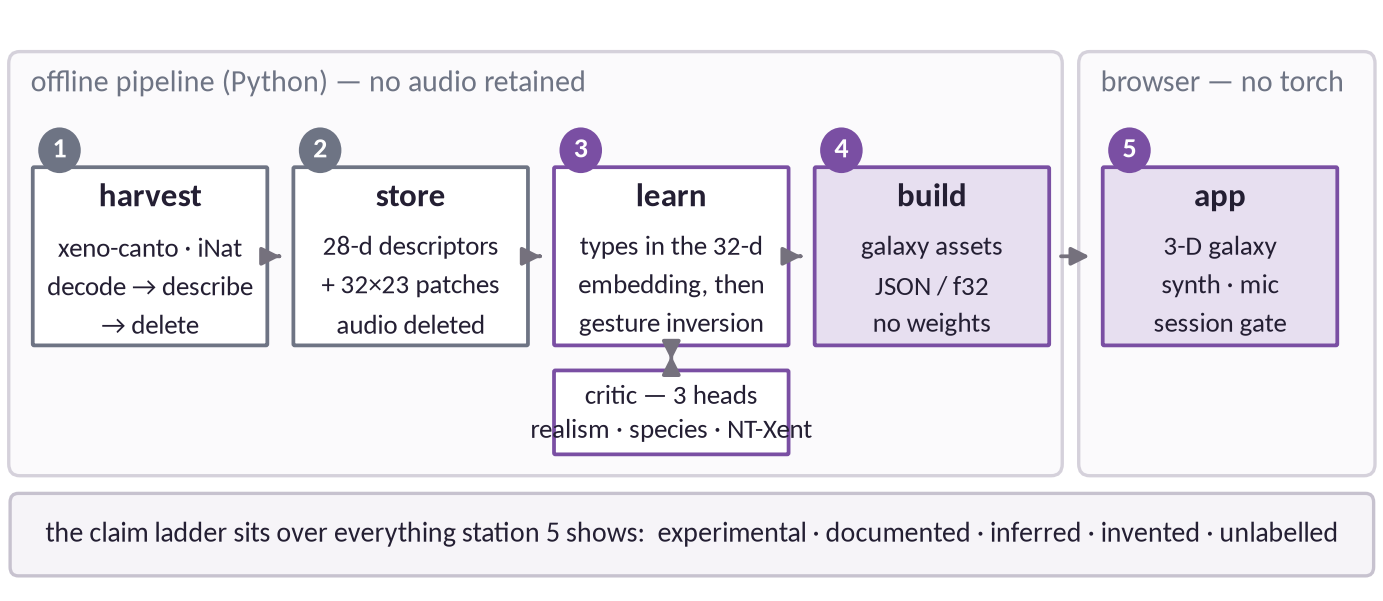
\includegraphics[width=\linewidth]{architecture.png}
\caption{The system end to end. Stages 1--4 are offline and are the subject of
Sections~\ref{sec:system}. Stage 5 reads static JSON and \texttt{float32} assets. The
evidence labels of Section~\ref{sec:premise} sit over everything stage 5 displays.}
\label{fig:architecture}
\end{figure*}

\subsection{Harvest: decode, describe, delete}

The harvester fetches from xeno-canto and iNaturalist through one loop that decodes a
recording, segments it, describes every syllable, and deletes the file; peak memory is one
recording. What is retained per syllable is a 28-dimensional descriptor, a
$32 \times 23$ log-mel patch (736 numbers, log-magnitude only, no phase), a four-knot
mel path, a duration, a pitch contour and provenance fields.
% docs/09 §9.3, §9.4

The corpus grew in four documented steps: an original 22-species store of 39\,976
syllables; a re-harvest carrying patches; a 121-species multi-source ingest; an
iNatSounds pass adding 6\,453 recordings, 226\,264 syllables and 3\,811 species in one run;
and a depth harvest adding 139\,440 syllables and taking recordings from 7\,992 to 10\,184.
The depth harvest targeted 100 species chosen for documented syntax cases, repertoire depth
and existing playback anchors, at up to 30 recordings each. It reached a median of 29
recordings per species on those 100, with 71 above the 20-recording threshold the syntax
work needs. The tenth percentile is 5, and that is the archive's ceiling rather than the
harvest's: xeno-canto holds no more for those birds.
% docs/16 §16.1; HANDOFF 2026-07-31 (P0)

Audio retention was later permitted where the licence allows it, for one measured reason:
an external model and any per-syllable re-measurement need the waveform. NoDerivatives is
refused, because everything downstream produces derived measurements, and an unrecorded
licence is refused, because absence of a licence is not permission. On the production store,
90.3\,\% of 10\,184 recordings pass and all 10\,184 carry a recordist. Nothing is shipped to
the browser.
% AGENTS.md hard constraints, owner decision 2026-08-01

\subsection{The 28-dimensional descriptor}

One descriptor per syllable offline, or per rolling window in the browser, computed
sample-for-sample identically on both sides; library defaults are not relied upon. Audio is
48\,kHz mono, peak-normalised to 0.9, framed at 1024 with hop 512 under a symmetric Hann
window. A frame is voiced if its unwindowed RMS exceeds $10^{-4}$ and 5\,\% of the clip
maximum. Per voiced frame: 13 mel-frequency cepstral coefficients from 26 triangular
filters on the power spectrum with energies floored at $10^{-10}$ and an unnormalised
DCT-II; the spectral centroid as $\log_2$ Hz; and spectral flatness. The descriptor is the
mean of the 13 coefficients, their population standard deviations, the mean $\log_2$
centroid and the mean flatness, standardised against corpus statistics shipped with the
assets.
% docs/08 §8.2

\subsection{The critic: one network, three heads}

Everything else in the pipeline is hand-written \textsc{numpy}. Two quantities, however, are
distances rather than physics, and hand-designed distances kept failing. A small
convolutional network on the log-mel patch carries three heads off a shared 32-dimensional
penultimate layer: a realism logit (real audio against our own resynthesis), a species
classifier over the training species, and a contrastive head under a
normalised temperature-scaled loss at $\tau = 0.2$ \citep{simclr2020}. Species are held
out entirely for the realism evaluation, because a network that has seen every species can
report identity instead of realism. Augmentations are small time stretches, gain changes
and added noise --- never pitch shifts, since pitch is type-diagnostic here.
% docs/09 §9.2b; critic.py docstring

Forcing all three tasks through one 32-dimensional bottleneck is the point: the embedding
has to answer all three at once. The production critic trained on 2\,686 species with 895
held out reaches realism AUC 1.000 on held-out species, species accuracy 0.730 over 2\,686
classes against chance 0.0004, and novelty ROC 0.846 flagging 32.2\,\% of unheard species'
syllables at a chosen 5\,\% false-positive rate.
% docs/16 §16.2; HANDOFF 2026-07-30

The network never generates. It scores, embeds and flags novelty; what ships is an
interpretable parameter vector rendered by the physical model.

\subsection{Typing, and the fit}

Syllable types are $k$-means clusters in the 32-dimensional embedding, with $k$ chosen per
species by silhouette. Replacing the previous hand-weighted seven-number observation vector
with the embedding is the largest single accuracy gain in the project
(Section~\ref{sec:internal}).

Each type is then fitted to the oscillator. The cluster median supplies a measured pitch
contour, duration, timbre class, attack and modulation depths. Coordinate descent
(\texttt{invert\_gestures}) then searches thirteen gesture axes --- including
\texttt{gammaScale}, \texttt{tractQ}, \texttt{noise} and \texttt{rough} --- over three
passes, a few hundred renders per type, moving only on an improvement. Measured contour and
duration are excluded from the search deliberately: the pitch tracker reaches them to about
1\,\%, and a search should not overwrite a measurement.
% docs/09 §9.3 Part 2; inverse.py docstring

The objective is a cosine between the resynthesis's 28-dimensional descriptor and the
type's mean-member reference, in the standardised harvest population frame. That single
scalar decides the gesture search, the respiration and two-voice ship gates, and the
fricative routing. Section~\ref{sec:walls} reports that it does not rank audible fidelity.

Two per-species fits sit beside the per-type one. The tracheal comb's fundamental $f_1$ is
\emph{measured}, not searched: per-syllable cepstral means are averaged over all of a
species' observations, inverted to a 26-band log spectral envelope, detrended, and scanned
for the $f_1$ whose odd-harmonic series best aligns with the residual. Because those
syllables span many recordings and a wide pitch range, pitch-dependent structure averages
away and only resonances fixed in hertz survive --- the long-term-average-spectrum argument
applied to a store that kept no audio. The measurement proposes and the resynthesis
decides: a species whose recordings show no tracheal colour keeps none. Implied effective
tube lengths came out at 1.7--6.6\,cm against 3.4--4.5\,cm measured in the
literature.
% docs/08 §8.1a

\begin{figure*}[t]
\centering
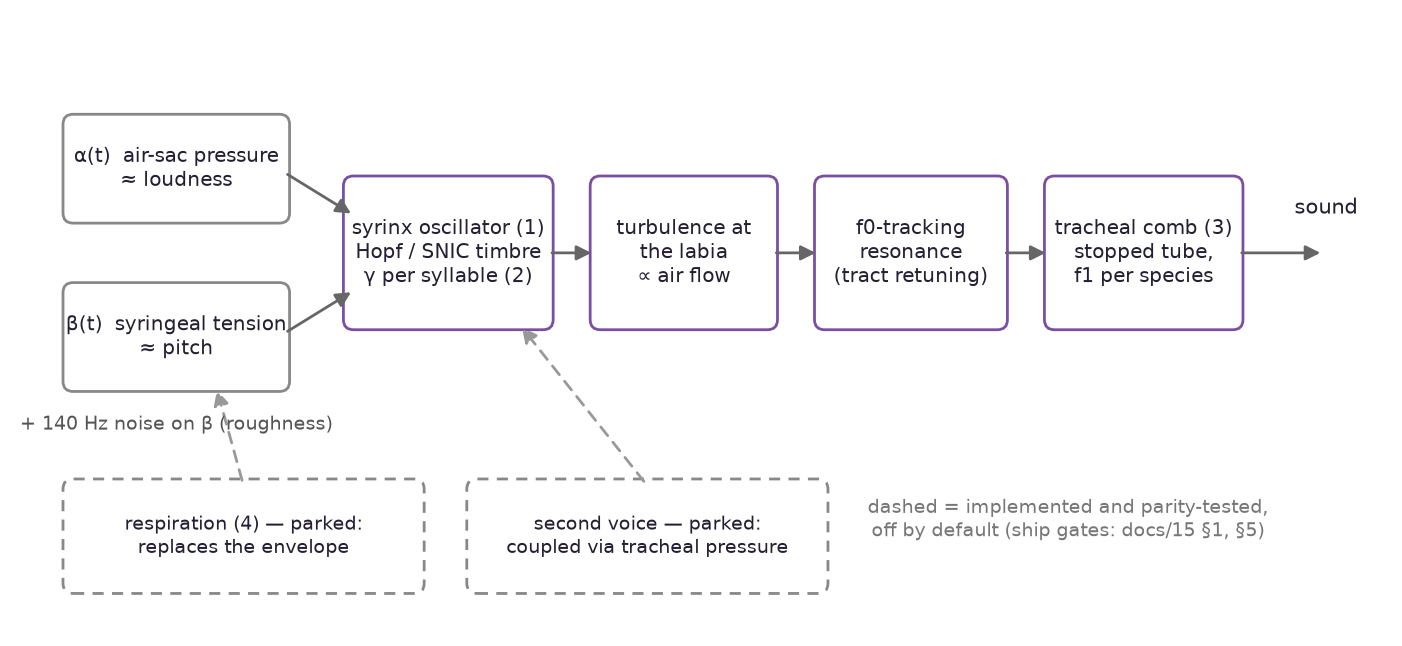
\includegraphics[width=\linewidth]{signal-chain.png}
\caption{The synthesis chain. Two gesture contours drive the oscillator; turbulence, the
$f_0$-tracking resonance and the fixed tracheal comb shape the result. The dashed blocks are
implemented, parity-tested and off by default: their published physics is not in doubt, but
their hand-set default parameter sets lost their pre-registered bake-offs, and only the
per-species fits ship, per type, where they win.}
\label{fig:signalchain}
\end{figure*}

\subsection{Grammar and songs}

A gap longer than 1.0\,s breaks a bout; that constant is shared by the grammar, the chunk
miner, the bake-off and the song detector through one named parameter, after a period in
which it existed as three separate literals. The shipped grammar is a first-order
transition table with Kneser--Ney continuation-count backoff \citep{kneser1995}, plus
26\,897 measured per-transition gaps, so nothing about the rhythm is invented.
% docs/22 §22.4; docs/16

Song types are detected rather than authored. Each bout's repeat runs are collapsed, the
collapsed strings are clustered by normalised edit distance, and a cluster of at least six
occurrences becomes a \emph{motif} song type. A second class was added after the funnel was
counted: a \emph{repeat} class is one collapsed string heard at least six times in bouts of
at least three syllables, matched by equality, because equality is the only similarity a
one-token string carries honestly. Both classes ship with a \texttt{kind} field so nothing
downstream has to infer which claim is being made. Every configuration is judged against a
within-species permutation control that keeps bout lengths and token marginals.
% docs/22 §22.1, §22.2; docs/12

\subsection{The map and the live path}

The build projects the 32-dimensional embedding to three dimensions, clusters it, and
writes plain JSON and \texttt{float32} assets: one position per syllable, per-cluster
centroids with labels, functions, confidences and citations, and the cross-species
relations document. Three clustering modes exist. The default is seeded $k$-means, where
each type contributes a seed and the resulting partition votes a name back by point-count
majority. HDBSCAN is the discovery mode, and is the only one that can answer ``none of
these''. Label assignment sends every point that already carries a type to its own type's
cluster and fits $k$-means only over the unlabelled remainder; Section~\ref{sec:internal}
reports what that is and is not worth.

The browser cannot run the critic --- no weights ship, which is a hard constraint rather
than a packaging detail --- so the live path needs a bridge from the 28-dimensional
descriptor it can compute to the 32-dimensional space the map lives in. That bridge is a
kernel ridge over random Fourier features ($D = 2048$, $\sigma = 4$, $\lambda = 1$),
fitted offline and shipped as plain numbers \citep{rff2007}. It is gated on held-out
\emph{recordings}, never on held-out syllables, because two syllables of one bird in one
take are nearly the same pair twice. A linear ridge came first and was replaced by
measurement, not by preference: it cleared the 0.8 gate at 0.8585 on a 19-species critic
and fell to 0.7997 once the embedding grew finer.
% docs/20; spacemap.py docstring

Live activation is a cosine against every centroid, a softmax at a shipped temperature, and
an exponential moving average at $0.82/0.18$, which is about 120\,ms of smoothing at
60\,Hz. A per-point brightness term makes a cluster light from the inside out --- the
members nearest the live sound brighten first --- so an active region shows its internal
structure instead of switching on as one blob.
% docs/08 §8.2; app/src/lib/galaxy/shaders.ts

\subsection{Verification}

The two renderers must agree sample for sample. A parity harness renders a fixture list
through the real AudioWorklet and through the Python renderer and compares them; it stands
at 18 of 18 fixtures with the worst divergence at float32 rounding
($2.8 \times 10^{-8}$). Six divergences had accumulated before it existed, including
amplitude modulation applied twice in the browser and a per-integration-step clamp that
flattened the high-amplitude regimes. A separate check renders all 44 authored syllables and
measures pitch, currently at 0.3\,\% median error. Forward Euler is validated against
Runge--Kutta to within 2\,\% of $f_0$, and the calibration table reproduces the reference
oscillator measurements to 0.1\,\% on $f_0$ and 2\,\% on peak-to-peak amplitude. The
noise generator is part of the contract: xorshift32 with a specified seeding rule, so that
``the same turbulence'' is a claim two implementations can be tested against.
% docs/08 §8.1, §8.1a; HANDOFF 2026-08-01; docs/21 §21.1

\begin{figure*}[t]
\centering
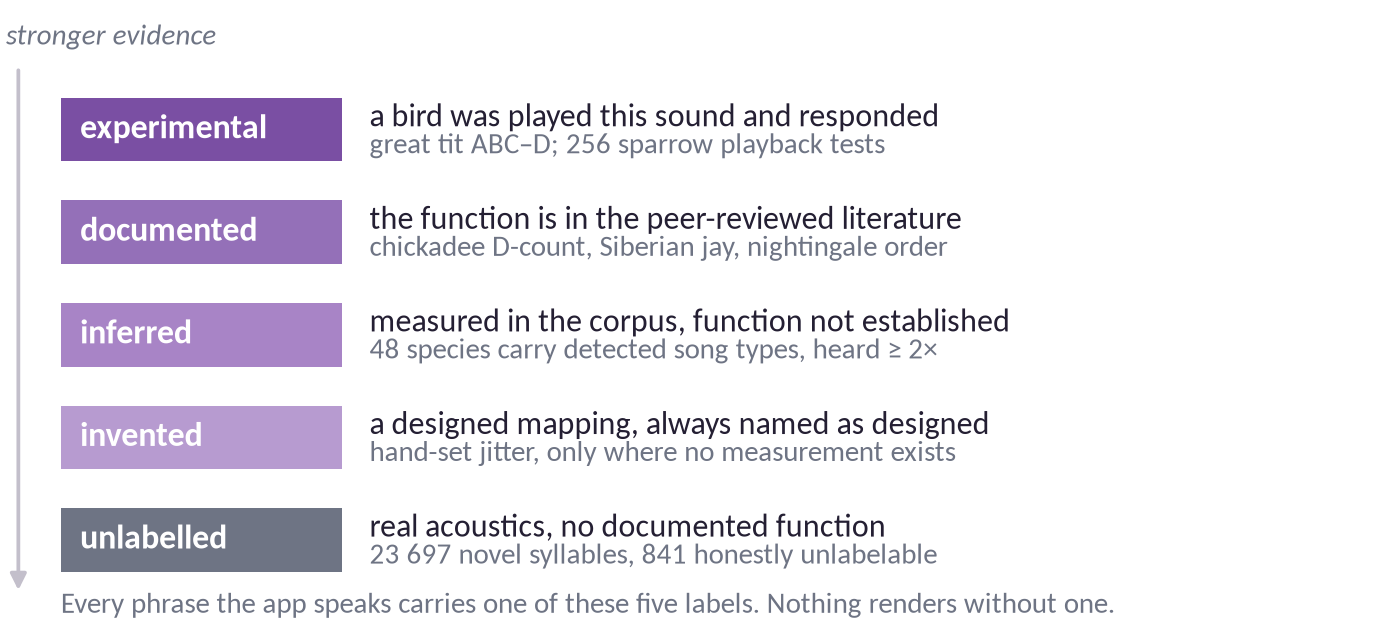
\includegraphics[width=\linewidth]{claim-ladder.png}
\caption{The five evidence labels, the requirement for each, and the corpus counts at the
time of writing. Every phrase the application speaks carries one of them; nothing renders
without one.}
\label{fig:claimladder}
\end{figure*}

% =====================================================================
\section{What is done differently, and where it stops}
\label{sec:walls}

\subsection{The contribution, stated plainly}

Four things here are not standard practice in this area.

\emph{A physical inventory at archive scale.} 13\,859 syllable types across 2\,421 species,
each one an interpretable parameter vector for a published oscillator rather than a latent
code. To our knowledge no comparable inventory exists; the physical-model literature fits
individual birds.

\emph{A corpus that is a description rather than a copy.} The store holds no audio and
cannot be inverted to recognisable audio, which changes what can be shared and removes the
licensing question from the analysis entirely.

\emph{Evidence labelling as an enforced invariant.} Five levels, applied to every rendered
phrase and every named region, with the ``unlabelled'' level protected: detecting that a
sound is new is not knowing what it means, and the interface is required to keep saying so.

\emph{Pre-registration as the working method.} Fifty-eight gates, written before their runs,
with the refusals kept in place. This is why the rest of this paper can be specific about
what the data does not support.

\subsection{Wall 1: the objective cannot hear}

The pipeline's universal fit objective is a 28-dimensional descriptor cosine. Measured
against two independent audible-distance metrics on 200 fitted types --- mel-cepstral
distortion \citep{kubichek1993} and multi-resolution log-spectral distance --- it carries
essentially no information: Pearson $+0.106$ and Spearman $+0.100$ against MCD, Pearson
$+0.102$ and Spearman $+0.111$ against STFT error. Neither is distinguishable from zero and
both point estimates lean the wrong way. This is not an instrument artefact: the recomputed
cosine reproduces the stored one at Pearson 0.921, and the two distortion metrics agree with
each other at 0.925.
% docs/19 §19.2 — n = 200 types, debug-100 store against the iNat audio cache

\begin{figure*}[t]
\centering
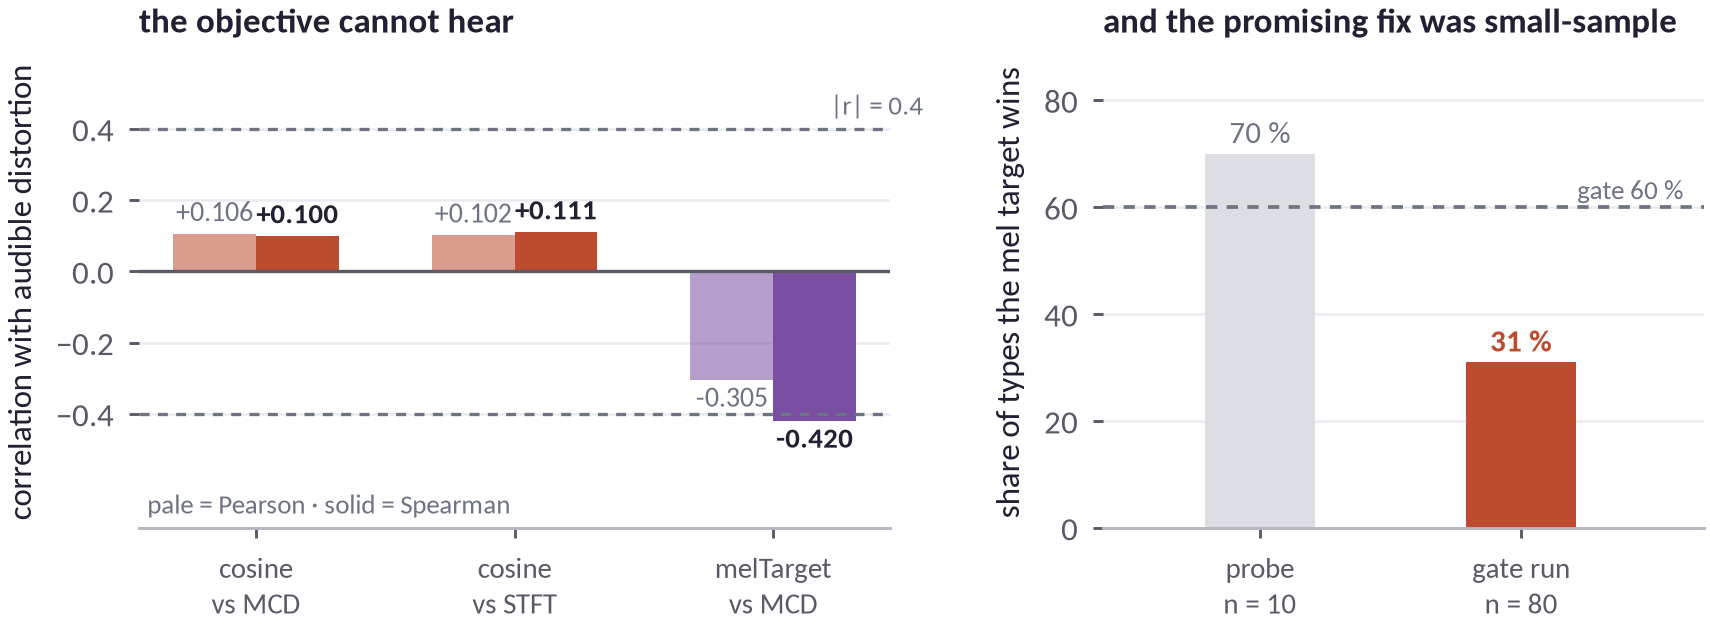
\includegraphics[width=\linewidth]{ruler.png}
\caption{Left: correlation with audible distortion for the incumbent objective and its
proposed replacement, $n = 200$ types on the 100-species debug store against the cached
audio. Right: the replacement's win share at exploratory scale and at pre-registered gate
scale. Both panels are debug-scale.}
\label{fig:ruler}
\end{figure*}

The mechanism is legible. High-cosine types are clean whistles whose renders concentrate
energy in one band while the field audio carries broadband noise everywhere else, so the
spectral distance is large; noisy buzzes score a low cosine but have broadband energy on
both sides, so the distance is small.

The obvious replacement was tried and does not work as an optimiser. A time-resolved mel-path
target correlates with MCD in the right direction and at usable strength (Pearson $-0.305$,
Spearman $-0.420$), which is what a fidelity ruler should do. Blended into the objective at
weight 0.5 it wins 31\,\% of types on MCD against a pre-registered 60\,\% bar, with a median
$\Delta$MCD of exactly 0.0\,dB and a maximum cosine loss of 0.120. A ten-type probe had won
7 of 10; the 80-type gate run settled it.
% docs/19 §19.4, §19.5 — n = 80, pre-registered gate

The honest state is therefore that the project measures spectrally and optimises
descriptor-wise. Every cosine-gated adoption in the system inherits that caveat, which is
recorded rather than hidden: the respiration and two-voice fit winners, the fricative
routing and the one-tone texture re-fit were all decided by a proxy that does not rank
audible fit at type level. They are not necessarily wrong --- each also improved the
descriptor match --- but ``improved the proxy'' is a weaker claim than it reads.

\subsection{Wall 2: the recordist, not the bird}

In the critic's embedding, the strongest relation is not the animal. Nearest-neighbour lift
over a permutation null, blocked by recording, is $+0.488$ for recordist and $+0.196$ for
species.
% docs/14 §14.4, production store
Every consumer of the embedding inherits that: typing, the map, the relations document,
novelty and the unknown-bird path.

\begin{figure*}[t]
\centering
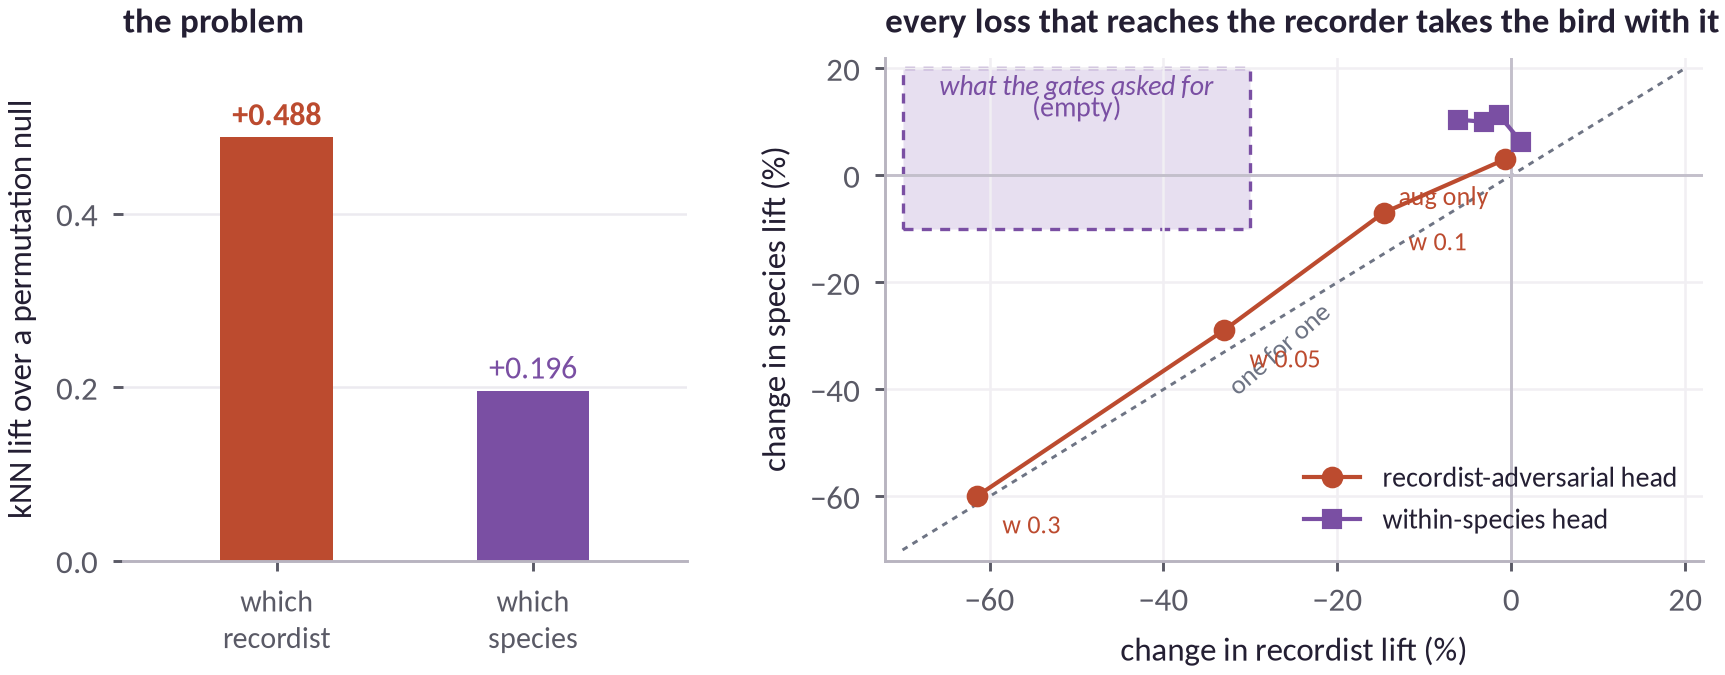
\includegraphics[width=\linewidth]{confound.png}
\caption{Left: what the embedding organises by. Right: every swept point from both
adversarial heads, as relative change in recordist lift against relative change in species
lift. The shaded region is what the pre-registered gates asked for and no arm reaches it.
37-species debug store; debug-scale.}
\label{fig:confound}
\end{figure*}

The road out has now been closed at four independent ends, which is
Section~\ref{sec:internal}'s and Section~\ref{sec:external}'s subject and is summarised here.
Training-time augmentation that simulates a recorder's frequency response moves the
recordist lift by $-0.7\,\%$, i.e.\ not at all. A gradient-reversed recordist head
\citep{ganin2016} does move it, at an almost exactly one-for-one cost in species structure.
A species-factored version of that head protects species completely and reaches only
$-6\,\%$ of the confound. Post-hoc batch correction, including the strongest member of the
genomics toolkit \citep{korsunsky2019}, reproduces the same one-for-one exchange rate by a
completely unrelated mechanism. And two archive-scale external models, neither of which has
ever been asked to tell our resynthesis from a bird, still carry between five sixths and
more than all of the recordist structure that ours does.

The reason is now visible and is a statement about the sample rather than about any model:
most species in this corpus are carried by a handful of recordists, so no method that sees
only the embedding can separate labels the data never separated. Subtracting each
recordist's mean leaves the recordist lift \emph{higher} than it started (0.1665 to 0.1687)
while costing a third of the species structure, so the confound is not a location shift and
not a per-dimension gain either.
% docs/23 §23.1.1
The named action is more recordists per species, in the data.

\subsection{Wall 3: syntax is data-limited, not method-limited}

A first-order transition model over the learned tokens is strongly supported
(Section~\ref{sec:findings}). A second order is not, and the reason is countable: of 2\,421
species, 217 clear the 20-bout bar at which the question can be asked at all. Within those,
the median species \emph{loses} 0.091 bits per token going from order 1 to order 2 on bouts
it has not seen, at three independent splits.
% docs/23 §23.2.2
The literature is unambiguous that birdsong is not
first-order \citep{jin2011,lu2025}, so this is a statement about the corpus, not about
birds. The depth harvest is the action, and it has a hard ceiling: the tenth percentile of
the 100 deepest species is 5 recordings, which is what the archive holds.

\subsection{Wall 4: the map's own confusion}

Two ceilings sit on the claim ``sing, and the right region lights''.

The first is in the embedding. With every type granted its own cluster --- so that no type
can fail to be retrieved for lack of a cluster --- the share of labelled points whose
nearest centroid by cosine belongs to their own type is 0.602. For 40\,\% of points the
nearest centroid is another type's. That is the embedding's confusion between types, not
the clustering's, and it was invisible until label assignment removed the competing
explanation.
% docs/22 §22.8, debug-100 fixed matrix, 214 154 points, 2 143 types

The second is in the bridge. On held-out recordings, the share of syllables whose nearest
region is the same through the ridge map as through the critic itself is 0.61 on the debug
build and 0.66 on production. Decomposing 1\,439 flips over 3\,731 held-out syllables
locates it: 76.4\,\% is boundary near-ties, with 74\,\% of all rows sitting inside a margin
of 0.05 and 41\,\% of flips landing on the runner-up region. Genuine large-margin map
failure is 4.3\,\% of the loss. Tie-adjusted agreement is 0.91 and species-level agreement
is 0.781 against chance 0.033. The consequence adopted was to make the honest single-label
claim at species level and to label region-level claims as ``nearest of several close
regions''; no better map class was pursued, because the addressable loss is at most
2.6\,\% of rows.
% docs/20 §20.1, §20.2 — debug build

\begin{figure*}[t]
\centering
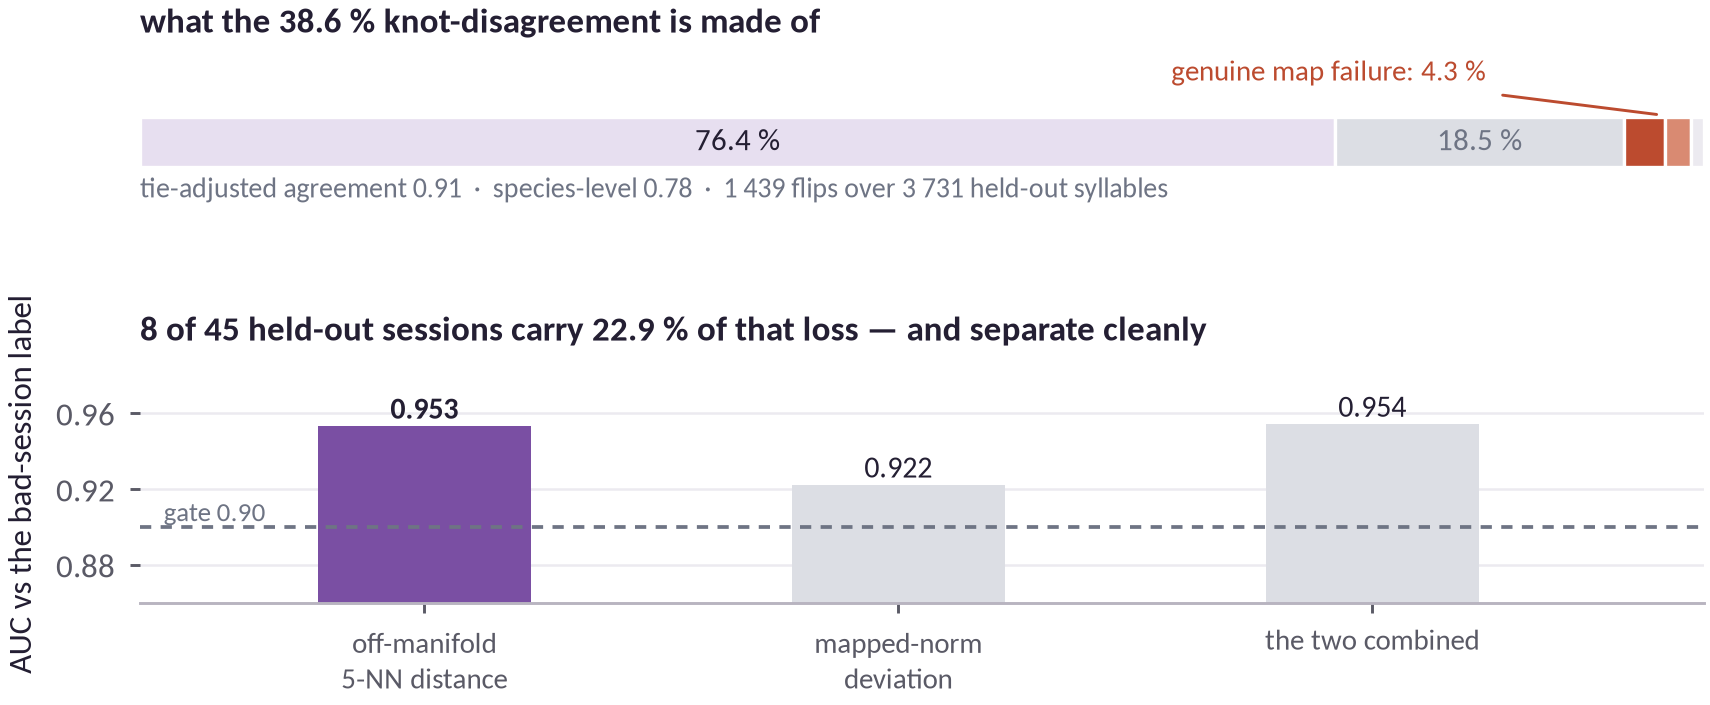
\includegraphics[width=\linewidth]{map-quality.png}
\caption{Top: the 38.6\,\% region disagreement between the browser's bridge and the critic,
decomposed over 3\,731 held-out syllables. Bottom: separation of the eight pathological
sessions by each candidate live signal, against the pre-registered adoption gate.
End-to-end debug build; debug-scale.}
\label{fig:mapquality}
\end{figure*}

\subsection{Wall 5: the fit, not the model}

An audit against the canonical literature found no deviation inside the oscillator
equations. The implemented ODE is the published normal form term for term, validated
against Runge--Kutta, against the reference oscillator measurements, against a two-sided
parity harness, and against the literature's own stated coupling-approximation boundary ---
the two-voice kernel's measured collapse into period doubling occurs exactly where
\citet{laje2005} says the weak-coupling approximation dies.
% docs/21 §21.1

Every recorded deviation sits outside the oscillator, and the list is specific. A single
$f_0$-tracking bandpass makes the spectral envelope pitch-invariant: measured relative
partial gains span 1.3-fold over a 5.7-fold change in $f_0$, against 32-fold for a fixed
waveguide, so the structure locks spectral shape to pitch. Pinning every syllable to
$\beta \approx 1$ places it at the tonal end of the model: the resynthesis reproduces the
median spectral content index almost exactly (1.099 against 1.092) and has essentially no
rich tail (1.4\,\% above 1.5 against 15.6\,\% of real syllables; 0\,\% above 3 against
5.3\,\%), with median spectral flatness three orders of magnitude too pure at 0.0005 against
0.044. The tension clamp bites in 6\,617 of 12\,724 types, so over half the corpus has
contour excursions riding a parameterisation limit while audible. Pressure arrives as a
designed envelope rather than as respiratory physics. And there is no physiological
micro-variation: real crystallised song carries about 1\,\% rendition-to-rendition
fundamental-frequency variation \citep{tumer2007}, and the implemented roughness mechanism
is one static fitted depth per type.
% docs/08 §8.1a; docs/21 §21.2; cli.py report_reachability

\begin{figure*}[t]
\centering
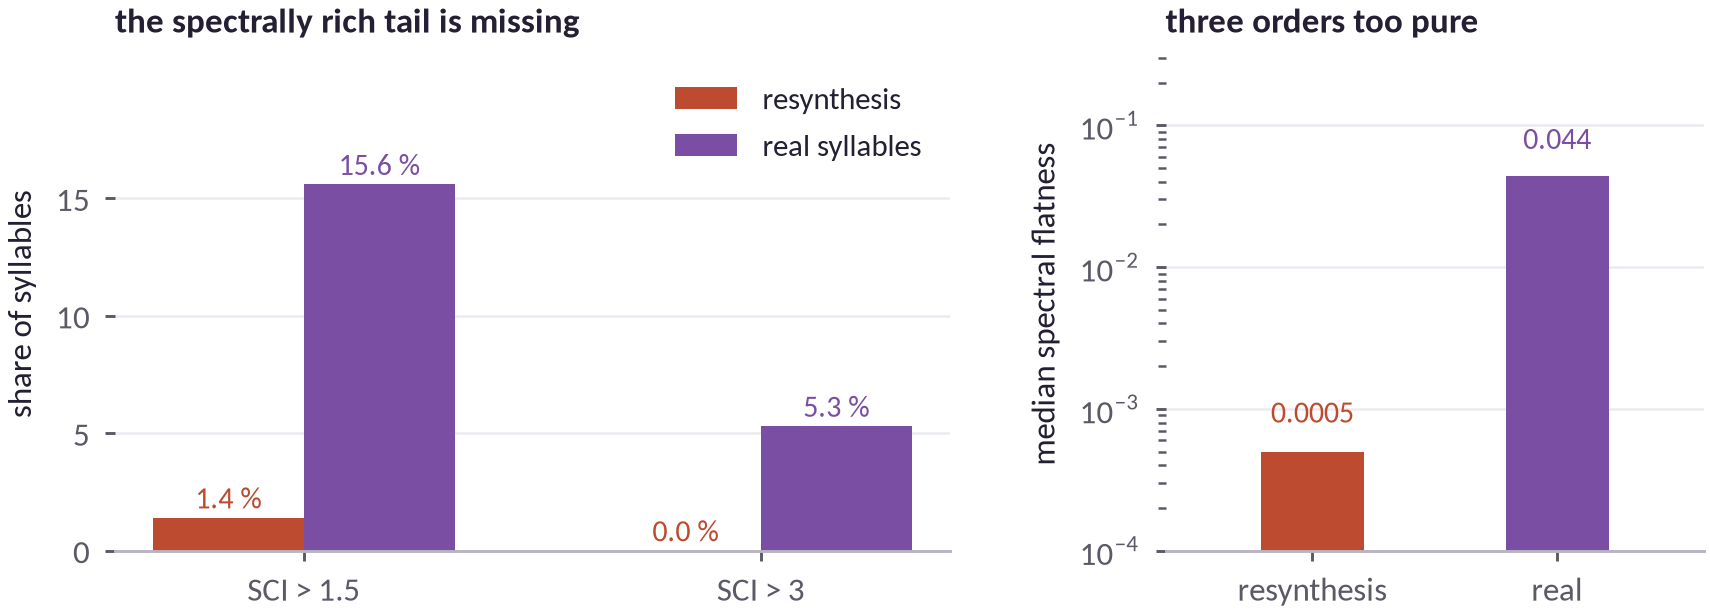
\includegraphics[width=\linewidth]{tonal-pin.png}
\caption{The tonal-regime pin. Left: share of syllables above two spectral-content
thresholds, resynthesis against real. Right: median spectral flatness on a log axis. The
model contains the pulse-like regime that produces the missing tail; the fit does not reach
it.}
\label{fig:tonalpin}
\end{figure*}

Two reading notes follow. First, ``noisy'' and ``machine-like'' are opposite failure modes
of one cause family: the representation has one noise axis and one envelope, so a fricative
collapses to unshaped hiss and a tonal note to a metronomic sine. Real syringes live
between the regimes, and the model contains that middle --- period-doubled and chaotic
solutions are in the equations \citep{sitt2008,amador2008} --- but the fit cannot find its
way there under the current objective. Second, the diagnosis is now sharper than ``the fit
fails'', because the starting point has been ruled out: an amortised inverse encoder that
proposes a full parameter vector in one forward pass reaches a comparable basin about as
often as the cluster median already does (Section~\ref{sec:internal}). What remains is the
objective and the physics beyond the oscillator.

% =====================================================================
\section{Our methods against each other}
\label{sec:internal}

This section reports the head-to-head arms the project ran against itself. Each states what
it licenses and what it does not. Unless noted, arms sharing a table were run on one fixed
corpus or one fixed dumped matrix, through the shipped functions rather than through
re-implementations, so they are comparable to each other and not necessarily to arms in
other tables. Throughout, ``points'' means percentage points: a retrieval score of 0.5775
rising to 0.6020 is $+2.5$ points.

\subsection{Hand-weighted typing against the learned embedding}

Syllable identity was originally decided by seven hand-weighted numbers. Replacing that
vector with the critic's 32-dimensional embedding is the largest accuracy gain the project
has measured. The headline metric is species placement: does a resynthesis land nearest its
own bird's centroid rather than another species'?

\begin{table*}[t]
\centering
\small
\caption{Typing space and fit objective, ablated on two stores. Each row changes one thing.
\emph{Species} is the share of resyntheses landing nearest their own species; \emph{cosine}
is the guardrail the critic cannot touch. Absolute values are not comparable between the two
panels: the stores differ, and the right-hand panel is a 13-species measurement after a
store-trim bug deleted twelve species, so chance there is 7.7\,\% rather than 4.0\,\%.}
\label{tab:typing}
\begin{tabular}{L{5.4cm} rrrr @{\hspace{1.2em}} rrrr}
\toprule
& \multicolumn{4}{c}{9\,041 syllables, 25 species} & \multicolumn{4}{c}{39\,993 syllables, 13 species} \\
\cmidrule(r){2-5}\cmidrule(l){6-9}
arm & types & species & cosine & $|f_0|$ & types & species & cosine & $|f_0|$ \\
\midrule
hand typing, cosine objective & 346 & 26.6\,\% & 0.762 & 5.4\,\% & 138 & 38.4\,\% & 0.807 & 3.3\,\% \\
\;+ realism objective, $w = 0.25$ & 346 & 27.2\,\% & 0.686 & 6.6\,\% & --- & --- & --- & --- \\
\;+ realism objective, $w = 0.50$ & 346 & 23.7\,\% & 0.655 & 6.5\,\% & 138 & 31.9\,\% & 0.642 & 4.0\,\% \\
\;+ realism objective, $w = 1.00$ & 346 & 17.3\,\% & 0.335 & 5.7\,\% & --- & --- & --- & --- \\
\textbf{learned-embedding typing} & 319 & \textbf{32.9\,\%} & 0.755 & 3.1\,\% & 294 & \textbf{51.7\,\%} & 0.796 & 2.2\,\% \\
hand typing $+$ waveguide tract & 346 & 30.1\,\% & 0.719 & 5.4\,\% & --- & --- & --- & --- \\
learned typing $+$ waveguide tract & 319 & 37.0\,\% & 0.706 & 3.6\,\% & 294 & 57.1\,\% & 0.723 & 2.1\,\% \\
\bottomrule
\end{tabular}
\end{table*}
% docs/09 §9.7 (9 k store), §9.8 (40 k store)

Table~\ref{tab:typing} licenses three statements and refuses a fourth.

Learned typing is a clean win, replicated on two stores at two species counts:
$+6.3$ points at 9\,k and $+13.3$ points at 40\,k, with the guardrail cosine essentially
held and pitch error improving in both. Nothing regresses.

The learned realism logit as a \emph{fit objective} is refuted, and it fails in exactly the
predicted way: monotonically harmful in its weight, with the cosine collapsing from 0.762
to 0.335 at $w = 1$ while placement drops to 17.3\,\%. A critic at realism AUC 0.990 on
entirely held-out species rules out ``the critic was not good enough''. Separating two
distributions is not the same as having a gradient that points at the nearer one. The
guardrail term earned its place by catching the thing it was put there to catch, and the
default weight is zero.

The own-type placement column, which we omit from the table, moves the wrong way as species
placement rises, and that is an artefact rather than a regression: the learned embedding
drove the type count from 138 to 294, and own-type placement asks whether a resynthesis
beats \emph{every other type of the same bird}. With twice as many rivals it is a strictly
harder question, and it is not comparable across rows with different type counts. That is
why species placement is the headline.

What the table does \emph{not} license is the waveguide row. A structurally fixed tract with
32 times the spectral freedom of the tracking band improves all three metrics at once on
five species and was a regression across 22 species on a different store; here it wins under
both typings and pays for it in cosine, missing the pre-registered guardrail. It remains
promising and unconfirmed, and it is gated off.
% docs/08 §8.1c; docs/09 §9.7

\subsection{Two spaces: the 28-dimensional descriptor against the 32-dimensional embedding}

The two spaces are not interchangeable and the choice is measured, not assumed. On a
controlled subset --- 625 field syllables, three species, identical points, one seed, only
the space changed --- moving the build into the embedding takes cluster purity from
70.9\,\% to 90.9\,\%, type coverage from 12/14 to 14/14, three-dimensional 10-nearest-neighbour
agreement from 64.5\,\% to 83.2\,\% and distance faithfulness from 0.874 to 0.940.
% docs/10 §10.2
On the 100-species debug corpus the descriptor-space discovery map degenerated to three
clusters with one holding 95\,\% of points --- iNaturalist soundscape audio is one density
blob in 28 dimensions --- where the embedding gives 98 clusters with real structure.
% HANDOFF 2026-07-31

Two honest counterweights sit against that. A render-free placement check scores the
32-dimensional space slightly \emph{below} the 28-dimensional one (38.5\,\% against
41.3\,\%), and the recordist confound of Section~\ref{sec:walls} lives in the embedding, not
in the descriptor. The embedding is the better similarity space and the worse-behaved one.
% docs/10 §10.2

\begin{figure*}[t]
\centering
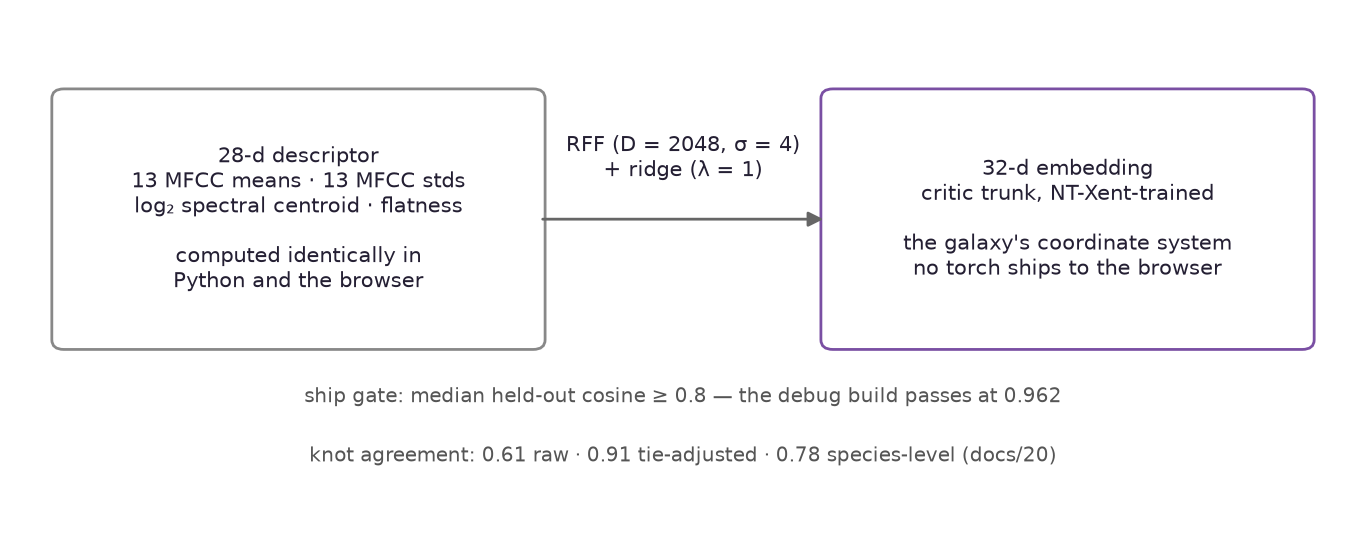
\includegraphics[width=\linewidth]{spaces-bridge.png}
\caption{The two feature spaces and the bridge between them. The browser computes only the
28-dimensional descriptor; the map lives in the critic's 32-dimensional embedding; a kernel
ridge over random Fourier features maps one into the other behind a ship gate on held-out
recordings.}
\label{fig:spaces}
\end{figure*}

\subsection{Objectives: cosine against a mel-path target}

Reported above in Section~\ref{sec:walls} and summarised here for the comparison table. The
mel target is the better \emph{measurement} and the worse \emph{optimiser}: it ranks audible
distortion where the cosine cannot (Spearman $-0.420$ against $+0.100$), and as an
objective at $w = 0.5$ it wins 31\,\% of 80 types against a 60\,\% bar with a median effect
of exactly zero. The two objectives agree only moderately on which types are good (Pearson
0.456), so they are complementary rather than redundant. An objective that is both a good
ruler and a good optimiser remains unfound.
% docs/19 §19.4, §19.5

\subsection{Clustering: seeded $k$-means against label assignment}

Ninety-six per cent of a production corpus's points already carry a
\emph{(species, syllable)} label by construction. The default build discards it, partitions
the space geometrically, and asks each partition to vote a name back by point-count
majority. Label assignment takes the other side of that design decision: every labelled
point goes to its own type's cluster and $k$-means fits only the unlabelled remainder.

All arms in Table~\ref{tab:clustering} run on one fixed matrix --- 214\,154 points, 2\,143
types, 160\,279 of the points from field recordings --- dumped from a 100-species debug
build, and every arm is scored through the shipped clustering, seeding and purity functions.
The harness was validated twice before any arm was read: the $k = 1024$ row reproduces the
earlier baseline exactly, and the $k = 4298$ row reproduces the shipped debug build's own
manifest.

\begin{table*}[t]
\centering
\small
\caption{Clustering arms on one fixed 100-species debug matrix (214\,154 points, 2\,143
types). \emph{Type retrieval} asks, for each point, whether the nearest centroid by cosine
--- the lookup the browser performs on live audio --- belongs to that point's own type.
Purity and coverage are identities under label assignment, not measurements. Debug-scale.}
\label{tab:clustering}
\begin{tabular}{L{6.6cm} r r r r r}
\toprule
arm & $k$ & purity & type coverage & type retrieval & clustering (s) \\
\midrule
$k$-means, uncapped (as shipped) & 4\,298 & 0.5797 & 0.9258 & 0.5775 & 64.9 \\
$k$-means at production's shed ratio & 1\,264 & 0.4601 & 0.5114 & 0.4599 & 25.5 \\
$k$-means at $k = 1024$ & 1\,024 & 0.4232 & 0.4260 & 0.4227 & 27.2 \\
\textbf{label assignment} & 4\,298 & \emph{0.9988} & \emph{1.0000} & \textbf{0.6020} & \textbf{0.2} \\
\bottomrule
\end{tabular}
\end{table*}
% docs/22 §22.8

The pre-registered gate asked for $+10$ points of type retrieval against the shipped
$k$-means build. It measured $+2.5$ and \textbf{failed}. The failure is the useful part. The
mechanism the gate was predicted from is types shedding their only cluster, and under the
raised cluster cap this corpus wants 4\,298 clusters and gets all 4\,298, so that mechanism
never fires. \emph{On a corpus that fits under the cap, seeded $k$-means is nearly as good
as knowing the answer} --- a real result about the seeding, and the argument against making
label assignment the default. Placing this corpus in production's shedding ratio
($k = 1264$) and at $k = 1024$ gives $+14.2$ and $+17.9$ points. The scope of the claim is
therefore exact: label assignment is worth what the cluster cap costs, and nothing more.

Two of the build's headline numbers stop being measurements under this arm. Purity 0.9988
and type coverage 1.0000 hold because a type \emph{is} a cluster here, by construction. The
shipped manifest says so in a dedicated field, because 1.0 read as a good map is reading the
definition back. Type retrieval is the statistic that survives, because nothing forces it.

There is a measured cost, and it is in the live path. Against the $k$-means build of the
same corpus, region-level agreement through the bridge falls from 0.6572 to 0.6316 and
species-level agreement from 0.7421 to 0.6831, while the tie-adjusted figure \emph{rises}
from 0.8032 to 0.8136. Read together that is more near-ties rather than worse decisions:
centroids placed at label means are less separated than centroids Lloyd's iteration pushed
apart, so more live sounds land between two regions --- and the ones that land decisively
land better. A build whose headline is the species claim should read that row first.
% docs/22 §22.8

\subsection{The synthetic member anchor (``W5'')}

The map was built out of both real and synthetic points: each type contributed one rendered
anchor plus renders of up to 24 measured member realisations, alongside the field syllables
those members already are. At production scale that made 51.1\,\% of the map a rendered copy
of the other half (347\,531 synthetic against 340\,079 field). Because the critic's leading
loss term is realism, the recorded/synthesised axis is the strongest relation in its
embedding (lift 0.990 against species' 0.513), so every type lived in two blobs and the
cluster budget bound at twice the type count.
% docs/22 §22.5

Three arms were run on the fixed matrix. Reducing member variants to the anchor alone moved
seeds per type from 2.000 to 1.993, i.e.\ not at all --- the source split is
\emph{binary}, splitting whenever a type holds points on both sides, so 24 renders and one
render split it equally. Deflating the source axis worked exactly as specified, removing
42.0\,\% of the space's energy and driving the gap between the two source means from 7.233 to
0.0, and \emph{every type still split} (1.999), with purity falling 1.1 points. So the
recorded/synthesised difference is not one direction: the global offset is, and the per-type
geometry the seeding gates on is not. What works is rendering nothing at all for a type
that has member observations, since it already exists in the map as the real syllables the
typing assigned to it: seeds per type falls to exactly 1.000 and the wanted cluster count
halves from 4\,298 to 2\,155.
% docs/22 §22.6

The follow-up changed what that arm is \emph{for}, and it is the cleanest methodological
lesson in this section. Type retrieval over \emph{all} points is not comparable between arms
that hold different points: dropping the synthetic copies drops the hard queries, so the arm
flatters itself by 18 points. Scored instead on the 160\,279 field points every arm holds
unchanged --- which is the population the question is about, since a recorded syllable must
light its own region --- the picture is different.

\begin{table*}[t]
\centering
\small
\caption{The same four arms scored on one query population: the 160\,279 field points every
arm holds unchanged. Label assignment is worth $+4.3$ points and is the same in both anchor
conditions, so the effect is the clustering's. Removing the synthetic anchor is worth
nothing on this statistic; what it is worth is half the regions and a quarter fewer points.
Debug-scale.}
\label{tab:w5}
\begin{tabular}{L{6.6cm} r r r r}
\toprule
arm & points & $k$ & field-point type retrieval & clustering (s) \\
\midrule
$k$-means, as shipped & 214\,154 & 4\,298 & 0.7176 & 54.8 \\
label assignment & 214\,154 & 4\,298 & \textbf{0.7604} & 0.2 \\
label assignment $+$ no synthetic anchor & 160\,579 & 2\,155 & \textbf{0.7606} & 0.1 \\
$k$-means $+$ no synthetic anchor & 160\,579 & 2\,155 & 0.7156 & 15.2 \\
\bottomrule
\end{tabular}
\end{table*}
% docs/22 §22.8, analysis/w5_field_retrieval.py

The anchor was removed on the size argument, not the accuracy argument, and the decision is
recorded as such. It halves the region count and removes a quarter of the points, taking the
production build from a wanted 27\,862 clusters to 14\,003 and the centroid asset from a
projected 44\,MB to 7.69\,MB of JSON plus 3.81\,MB of binary sidecar --- the difference
between ``needs a new asset format'' and ``ships''. It costs the rendered voice its own
place on the map, which is a claim about our synthesiser rather than about a bird. One
number moved the wrong way and it is a picture number: three-dimensional distance
faithfulness fell from 0.903 to 0.747 while 10-nearest-neighbour agreement rose from
20.7\,\% to 28.0\,\%. Removing 53\,575 rendered points removed structure the projection found
easy, so distance on screen means less than it did. Neither the regions nor the matching
ever used those positions.
% docs/22 §22.6 adoption note; HANDOFF 2026-08-01

\subsection{Where the descent starts: cluster median against an amortised inverse}

Coordinate descent starts each type's gesture axes at their defaults, which are wrong for
78\,\% of types on \texttt{gammaScale} alone. Since we own the forward model, training data
for an inverse is free: sample a parameter vector, render it, and measure the render with
the same patch function the critic consumes. This is the encoder-decoder arrangement of
differentiable DSP \citep{ddsp2020} with a physical decoder, which is why the
interpretability survives.

The gate was written before the encoder was trained, and both predicted weak spots were
recorded before the run: \texttt{tractQ} is the worst-learned head by an order of magnitude
(validation MSE 1.125 against \texttt{gammaScale}'s 0.102) and timbre classification reaches
0.442 over three classes where chance is 0.333.

\begin{table*}[t]
\centering
\small
\caption{The amortised inverse encoder as an initialiser, on two \texttt{learn} runs over
the 100-species debug store differing only in one flag. 1\,661 fitted types, all shared. The
gate was stated in full before the encoder was trained and fails on all three conditions.
Debug-scale.}
\label{tab:inverse}
\begin{tabular}{L{6.4cm} r r L{3.0cm}}
\toprule
& baseline & encoder & gate \\
\midrule
median resynthesis cosine & 0.7411 & 0.7546 \; ($+0.0135$) & $\ge +0.02$ \quad \textbf{fail} \\
mean resynthesis cosine & 0.6824 & 0.6997 \; ($+0.0173$) & --- \\
share of types improved & --- & 877/1\,661 $=$ 52.8\,\% & $\ge 60\,\%$ \quad \textbf{fail} \\
worst species' median change & --- & $-0.0816$ & $\ge -0.05$ \quad \textbf{fail} \\
\bottomrule
\end{tabular}
\end{table*}
% pipeline/analysis/inverse_gate.md

The median and the mean both rise, so the encoder does something real; it improves barely
more types than a coin would, and it costs one species a tenth of its fit. It is not
adopted, and the flag is off by default.

The finding that matters is diagnostic. \emph{The starting point was not the binding
constraint.} Coordinate descent from the cluster median already reaches a comparable basin
about half the time, which is more than the plan assumed when it described the search as
unable to escape a bad basin. So the remaining fit error is mostly not a basin problem, and
what is left of ``the model is right and the fit is what fails'' lives in the objective and
in the physics beyond the oscillator. The mechanism of the encoder's losses is visible in a
separate arm: an encoder-only start scores \emph{below} the cluster median it replaces (0.342
against 0.442), because on the fields the median already measures --- timbre, attack, hold,
harmonic, the modulations --- a regression estimate is worse than a measurement. Its only
new information is on the four gesture axes the median carries no value for, and the wins
cluster exactly there.
% inverse.py results table

A two-start variant was pre-registered in the same file rather than re-running the gate with
a softer bar: run the descent from both starts and keep whichever scores better on the
objective that already decides, which cannot regress by construction. Its bar is $+0.02$
median with \emph{no} species worse at all. Its measured cost is roughly 61 minutes against
the single-start arm's 11, because the encoder start explores a different basin and its
descent does not terminate as early.

\textbf{It passes, and it is the only pre-registered gate the inverse encoder has cleared.}
Median resynthesis cosine rises $0.7410 \rightarrow 0.7740$, a gain of $+0.0330$ against the
$+0.02$ bar; 51.7\,\% of the 1\,661 shared types improve, \textbf{none regress}, and no
species median falls (87 up, 13 unmoved, 0 down). Debug-100 subset, scored through the fit's
own per-type log against the baseline arm.
% arm A vs arm D, pipeline/analysis/inverse_gate.md; scorer analysis/score_two_start.py

The route there is worth reporting, because the gate's second condition earned its keep. The
first two-start run cleared the median bar at $+0.0320$ and \emph{failed} on 48 of 1\,661
types coming out worse, by up to 0.049. Since a two-start cannot regress by construction, the
pre-registration had already named that outcome a bug in the selection rather than a trade,
so it was diagnosed rather than excused. Three candidate explanations were eliminated by
measurement --- the search objective and the reported metric are the same computation; the
fricative refinement is monotone in its own input; the two arms fitted identical inventories
--- and a fourth by direct test: the renderer is bit-identical for fixed parameters, so the
reported cosine is a value and not a draw. The cause was that the selection compared
candidates \emph{before} the fricative refinement while the shipped and gated number comes
\emph{after} it, and that refinement's benefit depends on the basin: 19.3\,\% of types carry
the fricative flag, and 100\,\% of the 48 regressions did. Scoring each candidate as it would
ship took the regressions to zero and the median gain from $+0.0320$ to $+0.0330$.
% arm C -> arm D; 19.3 % vs 100 % of 48, p ~ 1e-35

Two limits belong with the number. It licenses a fit option that is never worse; it does not
license an audible claim, because the gate reads the same 28-d cosine whose correlation with
spectral distance is about $0.1$ (\S\ref{sec:ruler}), so a bench run on cached audio is what
an audible improvement would need. And the single-start arm's published worst-species figure
of $-0.0816$ was scored through the same pre-refinement comparison, so part of it is that
artefact rather than the encoder's fault --- which does not rescue that arm, since it failed
on the median alone.

\subsection{Grammar order on held-out bouts}

Four models, one protocol: per species, an 80/20 split by \emph{bout}, a $k$-order backoff
model fitted on the train half for $k = 0 \ldots 3$, every held-out token scored,
cross-entropy in bits per token. The corpus is 34\,696 bouts, 327\,164 tokens and 2\,421
species, of which 217 clear the 20-bout bar. The control is the same corpus with each
species' tokens redealt within species, keeping bout lengths and marginals. The loader is
pinned against the shipped bout function and refuses to run if the bout rule has drifted.

\begin{table*}[t]
\centering
\small
\caption{Held-out cross-entropy by Markov order, real corpus against its within-species
shuffle. 34\,696 bouts, 327\,164 tokens, 2\,421 species; 217 species clear the 20-bout bar.
The gate --- median gain $\ge 0.05$ bits/token at order $1 \to 2$, $\ge 0.05$ more than its
own shuffle, and share of species gaining $\ge$ control $+ 20$ points --- fails on the
magnitude criterion and passes on the share criterion, at three seeds.}
\label{tab:orders}
\begin{tabular}{L{7.4cm} r r}
\toprule
& real & control \\
\midrule
held-out cross-entropy, $k = 0$ (unigram) & 3.284 & 2.879 \\
$k = 1$ & \textbf{2.301} & 3.634 \\
$k = 2$ & 2.546 & 4.868 \\
$k = 3$ & 2.866 & 5.313 \\
\midrule
median gain, order $1 \to 2$ (bits/token) & $\mathbf{-0.091}$ & $-0.912$ \\
median gain, order $2 \to 3$ & $-0.108$ & $-0.187$ \\
share of species gaining at $1 \to 2$ & \textbf{25.3\,\%} & 4.1\,\% \\
\bottomrule
\end{tabular}
\end{table*}
% docs/23 §23.2.2, analysis/w2_heldout_orders.py

This table is the source of both the strongest positive result in the paper and one of its
clearest negatives, and Section~\ref{sec:findings} reads it in full.

A separate bake-off compared model \emph{classes} at first order and above. A
repeat-count-dependent model in the style of \citet{jin2011} lost decisively at $-0.348$
nats per token, winning 0 of 30 species. A hidden-state HMM won the pre-registered rule at
$+0.422$ nats and 29 of 30 species --- and the decomposition reversed the adoption. Splitting
held-out tokens by whether the transition was seen in training, first-order is the better
model on the 90\,\% seen ($-1.525$ against $-1.624$ nats/token, better in 15 of 30 species),
and the HMM's entire advantage is the 10\,\% unseen tail, where first-order pays $-9.25$ and
the HMM $-4.16$. That is a property of smoothing \emph{shape} --- a mixture predictive is
heavy-tailed --- not of recovered hidden structure. Adopting a heavier model for a smoothing
artefact would be the wrong lesson, so first order stayed and the smoothing was repaired
instead: a Kneser--Ney continuation backoff \citep{kneser1995} gains $+1.90$ and $+2.32$
nats per token on unseen-\emph{context} transitions across two debug stores with the seen
side bit-identical, and passes its own separately pre-registered gate. Two honest caveats:
80\,\% of the unseen tail is seen-context with an unseen continuation, outside the repair's
scope, so the full-tail gain is $+0.37$ and $+0.65$; and the repair narrows the HMM's
advantage, which confirms the diagnosis.
% docs/18 P1 and the backoff repair

\begin{figure*}[t]
\centering
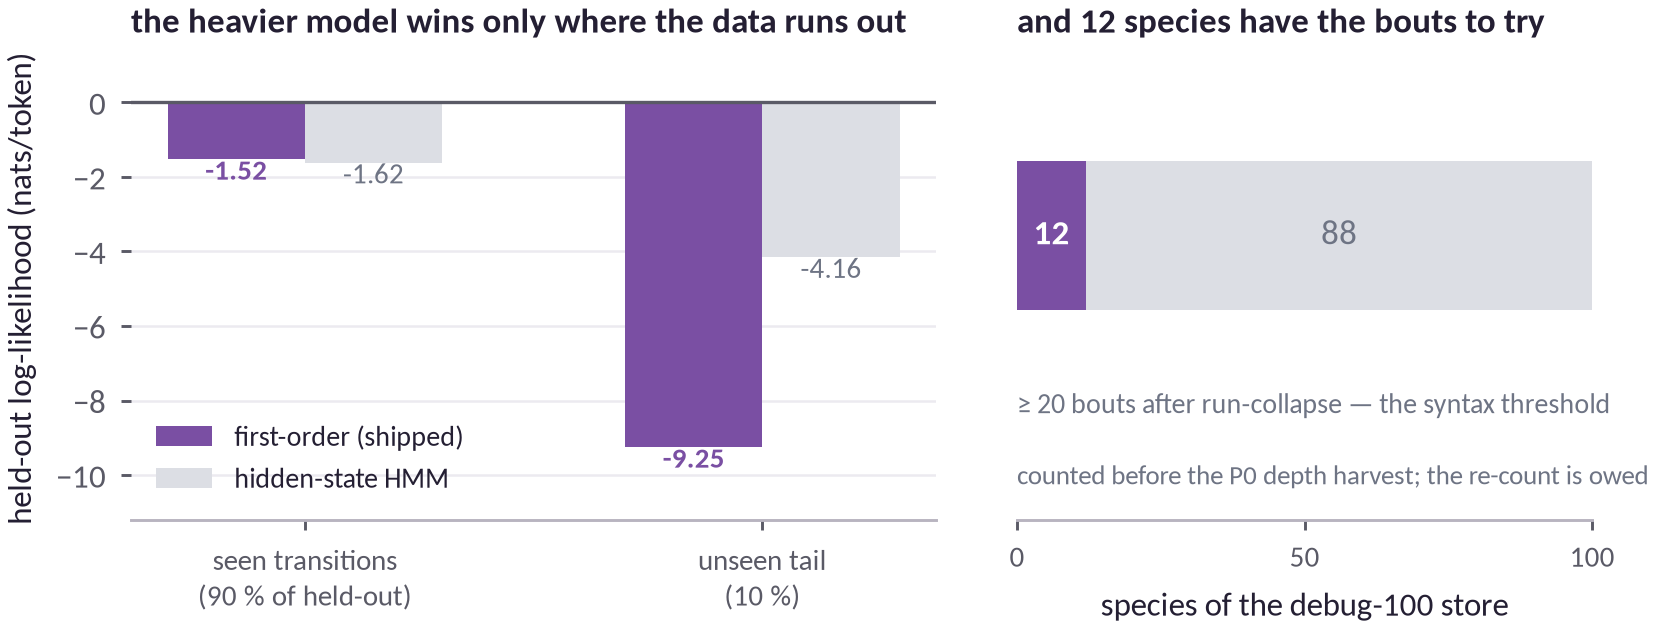
\includegraphics[width=\linewidth]{syntax-depth.png}
\caption{Left: held-out likelihood split by whether the transition was seen in training. The
heavier grammar's whole advantage lives where the data runs out. Right: species of the
100-species debug store with enough bouts to attempt song-level structure, counted before
the depth harvest. Both panels are debug-scale.}
\label{fig:syntaxdepth}
\end{figure*}

After the depth harvest the bake-off was re-run with qualifying species at 104 rather than
30. The HMM won again, at $+0.4976$ nats and 78 of 104 species, and this time against a
partially repaired baseline: subtracting the continuation backoff's own measured gain on the
same splits leaves the HMM ahead by about $+0.37$ nats per token. The debug-era explanation
cannot account for a residual that size, so something closer to genuine hidden structure is
scoring better now that the data can support it. It has \emph{not} been adopted: the shipped
inventory grammar is raw first-order counts, there is no HMM-state grammar writer, and
adopting one changes what the fit emits, what the application improvises from and what song
typing aligns against. That is recorded as the next syntax task with the number to beat.
% docs/18 P1 re-run 2026-08-01

\subsection{Song-level structure: an edit-distance kernel against bag-of-types}

Whole bouts as points, as (token, gap) sequences under a weighted edit-distance kernel with
the rhythm term priced inside the dynamic program, judged against plain bag-of-types over
the same bouts. It fails both pre-registered gates on both debug stores: species
nearest-neighbour lift $+0.877$ against bag-of-types' $+0.924$ on the 37-species store and
$+0.050$ against $+0.081$ on the 100-species store, with recordist lift $+0.264$ and
$+0.087$ against a $<0.05$ bar. Three measured details survive the failure. Within-species
song structure exists --- all 18 deep species separate their own recordings --- and lives
entirely in the token marginals, so order and rhythm add nothing measurable at current
depth. The rhythm term actively \emph{costs} species lift. And the bar for any learned song
encoder is bag-of-types, not the edit kernel.
% docs/18 P2

\subsection{Model-free sequence statistics against their own shuffle}

Three statistics that fit nothing, run on the production corpus against the same
within-species permutation control. Conditional entropy of the next token given one previous
is 0.941 bits against the shuffle's 3.343 --- not a subtle effect. The Menzerath--Altmann
exponent's median is $+0.019$ where the law predicts negative, with 45.7\,\% of species
negative against the control's 8.5\,\%: a weak effect in the law's direction, not the law, and
not the shape reported for geladas or penguins \citep{gustison2016,favaro2020}. The control's
own exponent is consistently positive, which is a sampling artefact rather than a finding --- a
mean over more draws sits closer to the species mean and its logarithm rises with the count ---
and that artefact is exactly why the control is run.
Normalised compression distance \citep{cilibrasi2005} is refuted outright, because the control
separates species \emph{better} than the real corpus does (0.038 against 0.018) ---
compression distance here reads alphabet and marginals, which the shuffle preserves, and
not order. No learned song encoder should be measured against it.
% docs/23 §23.2.1

One arm from this set was retracted by the project itself and is recorded as a design error
rather than as a result. Comparing the $k=1 \to k=2$ entropy drop between real and control
is not a valid test when the two curves start 2.4 bits apart, and past $k=3$ the control's
plug-in curve falls \emph{below} the real one because a plug-in estimator reports
near-unique contexts as determined. Both effects are bias. The verdict function now refuses
that comparison rather than returning the answer it would have returned, and the honest
instrument --- held-out cross-entropy, unbiased by construction --- is
Table~\ref{tab:orders}.

\subsection{Detector configurations against a permutation control}

Three configurations of the song detector were run against the same corpus-wide shuffle
control, whose yield bar was 0.2\,\% of candidate bouts.

\begin{table*}[t]
\centering
\small
\caption{Song-detector arms on the production store (2\,421 species, 34\,696 bouts, 10\,550
candidate bouts of three tokens or more). Only the first passes. The control yield is the
share of candidate bouts a within-species shuffle places, and the pre-registered bar is
0.2\,\%.}
\label{tab:songdetector}
\begin{tabular}{L{5.6cm} r r r r l}
\toprule
arm & species with a song & song types & placed bouts & control yield & verdict \\
\midrule
shipped, motifs only & 48 & 96 & 1\,052 & 0.170\,\% & baseline \\
\textbf{$+$ repeat classes} & \textbf{98} & \textbf{356} & \textbf{3\,741} & \textbf{0.170\,\%} & adopted \\
per-species recurrence bar & 99--202 & 452--636 & --- & 0.266--0.442\,\% & refuted \\
per-species bout rule & 105 & 449 & --- & 0.628\,\% & refuted \\
\bottomrule
\end{tabular}
\end{table*}
% docs/22 §22.2, §22.3, §22.4

Repeat classes pass on both halves of their gate and are adopted. The control is unchanged
to the bout, because shuffling a species' tokens destroys runs, so the control finds no
repeat classes at all --- the sharpest evidence available that the ones found are real.

The two refuted arms are instructive in the same way. Letting each species set its own
recurrence bar on the evidence of its own shuffled tokens let 2\,398 of 2\,421 species take
the loosest bar, because a species with eight candidate bouts has a control that cannot place
a bout at any size: ``the control found nothing'' meant ``the control had nothing to work
with''. Adding a power requirement repairs the mechanism but not the verdict --- no candidate
threshold in $\{10, 15, 20, 30, 50\}$ returns the control to 0.2\,\%, and the rows that come
closest gain almost nothing over the 98 species repeat classes already reach. A per-species
bout rule at five times the species' own median gap reaches 105 species at nearly four times
the chance yield, because splitting a fast singer's bouts finer produces more short strings
and short strings are what chance can chain. Both were removed with their flags: a refuted
policy nobody can reach is surface, not machinery, and the tables are what survive of them.

\subsection{What this section licenses}

Read together, the internal comparisons say four things. The choice of \emph{space} matters
most and is settled: the learned embedding beats the hand-weighted vector by 6 to 13 points
of species placement, replicated. The choice of \emph{clustering} matters exactly as much as
the region budget binds, and no more. The choice of \emph{objective} is unresolved and is the
project's central open problem: the best available ruler is the worst available optimiser.
And the choice of \emph{starting point} does not matter, which is a genuinely useful negative
because it eliminates one of the two remaining explanations for the fit's failure.

% =====================================================================
\section{Our methods against other approaches}
\label{sec:external}

\subsection{What is and is not a fair comparison}

The external comparisons in this section are all read-only tests on a fixed store, through
one estimator --- nearest-neighbour lift over a label permutation null, blocked by recording
--- with no training and no new data. That makes them directly comparable to every lift this
project has published. Three limits apply and are stated before the numbers, because they
change what the numbers mean.

First, \textbf{the representation is per recording, not per syllable}. Perch's point is the
mean of a recording's first six 5-second window embeddings; BirdNET's is the analogous
average of its 3-second windows; the critic's is the mean of that recording's syllable
embeddings. That form was chosen because two points from the same recording cannot exist in
it, so same-recording leakage is impossible by construction rather than by exclusion. But
the critic's embedding is a \emph{syllable} space being averaged over a recording, which is
not the job it was fitted for. So a species-retrieval result here says that an external space
is the better \emph{per-recording} descriptor. \textbf{It does not say that Perch or BirdNET
beats our critic syllable for syllable. That comparison has never been run.} The reason it
has not is recorded: a per-syllable Perch pass over 340\,079 syllables is about 3.3 hours on
this machine's CPU, the installed ONNX runtime does not match the installed CUDA version,
and the GPU provider fails to load and falls back to CPU silently at no measured speed
difference.
% docs/23 §23.6.1b, §23.6.2

Second, \textbf{the populations differ between the two draws and the difference is the
result}, not noise to be averaged away. One draw was built for the recordist question, one
for the species question, and they disagree about the recordist verdict. The tie-break was
fixed on coverage before the disagreement appeared.

Third, \textbf{the audio cache constrains what can be asked at all}. It holds at most two
recordings per species --- 2\,616 species with exactly two, 1\,221 with one, none with three
--- because the iNaturalist ingest took no more and the xeno-canto audio was deleted at
harvest by design. No species group of eight recordings exists on any audio this machine
holds, so a species-stratified draw returns zero recordings and no selection rule can produce
one. Anything needing several recordings of one species needs audio re-fetched first.
% docs/23 §23.6.1

\subsection{Recording-condition invariance: three spaces, two populations}

\begin{table*}[t]
\centering
\small
\caption{Recordist and species nearest-neighbour lift over a permutation null, for our
32-dimensional critic and two archive-scale external models, on two populations. Per
recording in every row; same rows and same null within each population. \emph{Coverage} is
the share of rows for which the estimate is defined. T1's gate asked for a 30\,\% relative
reduction in recordist lift; T3's asked for a species-retrieval improvement.}
\label{tab:external}
\begin{tabular}{L{4.2cm} r r r}
\toprule
space & dims & recordist lift & species lift \\
\midrule
\multicolumn{4}{l}{\textbf{T1 population}: 1\,567 recordings, 135 recordists, 1\,341 species; recordist coverage 0.907} \\
critic & 32 & 0.0891 & not estimable \\
Perch 2.0 & 1\,536 & \textbf{0.0744} \; ($-16.5\,\%$) & not estimable \\
BirdNET & 1\,024 & 0.1107 \; ($+24\,\%$) & not estimable \\
\midrule
\multicolumn{4}{l}{\textbf{T3 population}: 958 species with two recordings each, 1\,644 recordings, 760 recordists;} \\
\multicolumn{4}{l}{species coverage 0.834, recordist coverage 0.329} \\
critic & 32 & 0.1684 & 0.0074 \\
Perch 2.0 & 1\,536 & \textbf{0.1155} & \textbf{0.0588} \\
BirdNET & 1\,024 & 0.1755 & 0.0393 \\
\bottomrule
\end{tabular}
\end{table*}
% docs/23 §23.6.1, §23.6.2, §23.6.3

\textbf{T1 fails, and it is the fourth independent closure of the same road.} Perch 2.0 ---
trained on the same archives at roughly a hundred times our scale, never asked to tell our
resynthesis from a bird, and therefore structurally incapable of having learned the axis that
splits our types in two --- still carries five sixths of the recordist structure our own
critic carries. The gate asked for $-30\,\%$ and measured $-16.5\,\%$. The prediction was
written in advance and is worth quoting rather than softening: \emph{if a model trained on
the same archives at a hundred times the scale is no more recorder-invariant than ours, the
confound lives in the archives rather than in our critic.} It does.

\textbf{BirdNET fails harder, and the disagreement between the two external models is
stronger evidence than either alone.} BirdNET's recordist lift is \emph{above} our critic's
in both populations ($+24\,\%$ and $+4\,\%$). Perch reads $-16.5\,\%$ and BirdNET $+24\,\%$
on the same rows. If archive-scale training conferred recorder invariance, the two largest
models trained on these archives would both have it and they would agree. One is better than
ours and one is worse, which locates the property in the archives rather than in any model's
loss --- the same conclusion the batch-effect analysis reached from the inside, now reached
from outside with two independent instruments.

\textbf{T3 passes decisively, within its stated scope.} Perch retrieves a species' other
recording 8 times better than our critic does (0.0588 against 0.0074) and BirdNET 5.3 times
better (0.0393), on the same rows against the same null. The direction replicates across both
external models, so ``an external space is the better per-recording species descriptor''
holds. It licenses Perch as the per-recording batch descriptor for any future invariance
work, and it weakens the case for building further external ports to answer T1, which is
answered three ways.

\textbf{The finding that holds in both draws is the one to carry.} In Perch's space the
recordist lift is still twice the species lift; in BirdNET's it is 4.5 times; in ours it is
23 times. Every space tested is confounded in the same direction and they differ only in
degree. A model trained on these archives at a hundred times our scale, which has never seen
a resynthesis, still encodes \emph{who recorded it} more strongly than \emph{which bird it
is}.

Two things are explicitly not settled. T1's own verdict rests on a coverage tie-break: it
passes at $-31.4\,\%$ on the T3 population and fails at $-16.5\,\%$ on the T1 population,
and the T1 population's recordist estimate covers 0.907 of rows against the other's 0.329, so
the instrument built for the question wins and the verdict is fail. And the novelty
comparison --- Perch against our critic's novelty ROC of 0.846 --- was never run. Retiring
the critic's species head was made conditional on T1 \emph{and} T3 landing; T3 landed and T1
did not, so it stays.

\subsection{Post-hoc batch correction against training-time invariance}

The same confound was attacked with the genomics batch-effect toolkit, which has the property
that its strongest members are post-hoc: they correct an embedding that already exists.
20\,000 syllables of the production embedding, 885 species, 1\,001 recordists, 3\,265
recordings, every arm scored by the same estimator against its own null.

\begin{table*}[t]
\centering
\small
\caption{Post-hoc batch correction of the production embedding. 20\,000 syllables, 885
species, 1\,001 recordists, 3\,265 recordings. The gate asked for the recordist lift halved
with species lift not falling at all. No arm passes: every arm that halves one halves the
other.}
\label{tab:batch}
\begin{tabular}{L{5.6cm} r r r}
\toprule
arm & species lift & recordist lift & ratio \\
\midrule
baseline & 0.1643 & 0.1665 & 0.99 \\
centre by recordist & 0.1113 & 0.1687 & 0.66 \\
whiten by recordist & 0.0955 & 0.1540 & 0.62 \\
Harmony by recordist & 0.0501 & 0.0478 & 1.05 \\
centre by recording & 0.0432 & 0.0408 & 1.06 \\
whiten by recording & 0.0342 & 0.0331 & 1.03 \\
Harmony by recording & 0.0463 & 0.0501 & 0.92 \\
\bottomrule
\end{tabular}
\end{table*}
% docs/23 §23.1.1, batcheffect.py

Three findings, in increasing order of consequence. The confound is not a location shift:
subtracting each recordist's mean leaves the recordist lift higher than it started while
costing a third of the species structure, which is a mechanistic explanation for why two
training-time attempts failed and one that was never available before, because both of those
attacked the confound during training where nothing can be inspected. Harmony
\citep{korsunsky2019} reaches it and pays exactly the price a gradient-reversed adversarial
head paid: $-71\,\%$ recordist, $-70\,\%$ species. Two unrelated mechanisms landing on the
same exchange rate is evidence about the data rather than about either mechanism. And
correcting by recording removes both because the labels are nearly nested --- a recording
normally holds one bird of one species --- which is a statement about how the corpus was
collected.

Against that, the data road works and its effect size shrank honestly when re-tested.
Figure~\ref{fig:avex} shows both scales. Merging two genuinely different recording domains
--- iNaturalist soundscape and xeno-canto focal --- bought $+14.4$ points of cross-domain
species retrieval on the 12 species present in both stores, with a 3-species holdout. The
pre-registered bigger re-test on 63 both-domain species with 16 held out took that to
$+3.6$. A cross-domain contrastive mechanism on top reached $+13.4$ at the small scale and
$+1.7$ against a $+10$ gate at the larger one, so the mechanism's boost was small-sample
structure. The uncomfortable part is recorded plainly: the merge's \emph{own} win shrank too,
and its held-out realism AUC reads below the single-domain arm's here (0.976 against 0.995)
where the first test gained 0.012. Every number from the first test should be treated as
small-sample in both directions. What survives the bigger test is the ordering, which is the
load-bearing claim: more domains per species helps, and the mechanism adds approximately
nothing on top of the data.
% docs/17 §17.4, §17.6.1

\begin{figure*}[t]
\centering
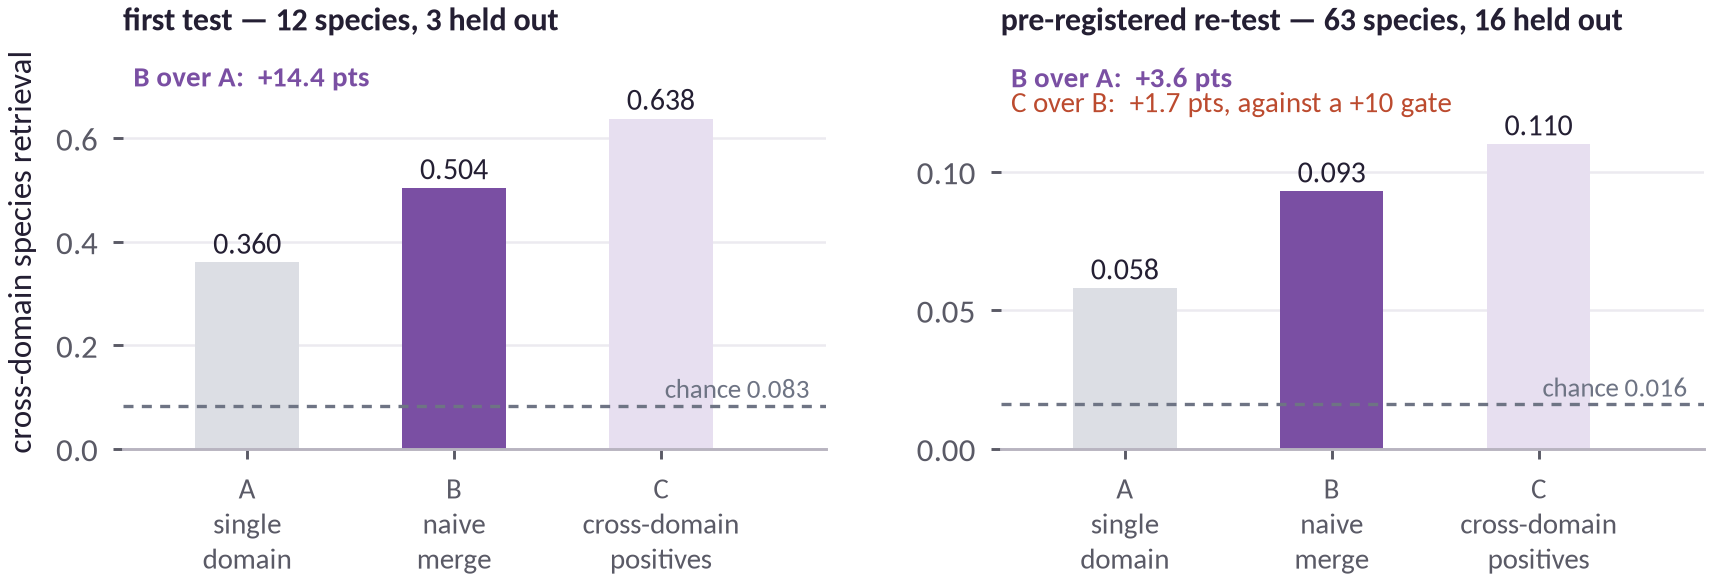
\includegraphics[width=\linewidth]{avex.png}
\caption{Cross-domain species retrieval for three training arms at two scales. Both panels
are debug-scale and absolute levels are comparable only arm against arm inside each panel.
The pre-registered re-test shrank every effect; the ordering survived.}
\label{fig:avex}
\end{figure*}

\subsection{Positioning}

Table~\ref{tab:positioning} places the system beside the approaches it is most likely to be
confused with. A cell reads ``not documented'' where the cited sources do not answer it; the
column entries for this work are properties of the shipped artefact, not aspirations.

\begin{table*}[t]
\centering
\small
\caption{Approaches beside each other. External rows are read from the cited sources;
``not documented'' means the source does not answer the cell. \emph{Interpretable
parameters} means a reader can name the quantity that produced a given sound.}
\label{tab:positioning}
\begin{tabular}{L{2.9cm} L{3.5cm} c L{2.5cm} L{2.6cm} c}
\toprule
approach & what it is & sings & interpretable parameters & runs as a static asset set & labels its claims \\
\midrule
BirdNET \citep{birdnet2021} & species classifier on spectrograms & no & no & no & not documented \\
Perch 2.0 \citep{perch2} & general bioacoustic embedding, ${\sim}15$k classes & no & no & no & no \\
AVES \citep{aves2022} & self-supervised animal audio encoder & no & no & no & no \\
BirdMAE \citep{birdmae2025} & masked autoencoder for bird audio & no & no & no & no \\
NatureLM-audio \citep{naturelm2024} & audio-language model for bioacoustics & no & no & no & no \\
\citet{sainburg2020} & projected latent space across repertoires & no & latent, not physiological & not documented & no \\
\citet{goffinet2021} & learned low-dimensional vocal features & no & no & not documented & no \\
generative audio models & waveform generators & yes & no & no & no \\
\textbf{Lyrebird} & physical syrinx $+$ a corpus with no audio in it & \textbf{yes} & \textbf{yes} --- pressure, tension, tract geometry & \textbf{yes} --- no audio retained, no weights shipped & \textbf{yes} --- five levels \\
\bottomrule
\end{tabular}
\end{table*}

The comparison that matters is not on accuracy, because the systems answer different
questions. The external models are better at ``which bird is this'', by a margin that has
been measured here at 5 to 8 times on per-recording species retrieval, and this work should
be read as taking that for granted rather than competing with it. What this work provides
that none of them does is a \emph{generative, physically parameterised} account of a syllable
that is fitted to field audio at archive scale, together with an explicit statement of the
evidence behind every claim built on it.

% =====================================================================
\section{What the data supports}
\label{sec:findings}

This section states what can be read out of the corpus, at what strength, with the ceiling
attached to each claim. Numbers from the 100-species debug subset are marked
\emph{debug-scale}; numbers from twelve-species or ten-type samples are marked as such,
because the project has twice measured an effect at small scale that did not survive
replication, in both directions.

\subsection{The tokens are units. This is the strongest result in the paper.}

A first-order transition model over the learned syllable-type inventory buys \textbf{0.98
bits per token} on held-out bouts --- cross-entropy 3.284 down to 2.301 --- while on a
within-species shuffle of the same tokens, with bout lengths and marginals preserved, the
same model \emph{costs} 0.75 bits (2.879 up to 3.634). The corpus is 34\,696 bouts, 327\,164
tokens and 2\,421 species; the estimator is unbiased by construction, which the plug-in
estimator this replaced was not.
% docs/23 §23.2.2

The logic is what makes it strong. An unbiased estimator paying for parameters it cannot use
is the clean form of the claim that the tokens are units: the model can only win if the
transitions are real, and it wins by a bit per token. This holds a load-bearing assumption
that everything above the syllable rests on. The syllable inventory is produced by $k$-means
in a learned embedding, which is a clustering; the question of whether it is also a
\emph{unit system} is not answerable by comparing two models, and it is answered here in the
affirmative. A model-free estimate on the same corpus agrees: conditional entropy of the next
token given one previous is 0.941 bits against the shuffle's 3.343.
% docs/23 §23.2.1

Two artefacts belong with the number. The control's unigram cross-entropy sits \emph{below}
the real corpus's (2.879 against 3.284), because shuffling spreads each species' tokens
evenly across its bouts so that train and test marginals nearly coincide, whereas real bouts
are clumped --- a bout tends to repeat one type --- so a held-out real bout can be mostly a
type the train half barely saw. That clumping is itself structure, and it is why the gate
reads within-corpus deltas rather than the two absolute curves against each other. And the
same behaviour is pinned in a self-test: a planted second-order process must be found, a
first-order process must not show depth, and the shuffle of the planted process must not gain
from a longer context.

\subsection{Repeat classes double the corpus's songs, with the control unmoved}

The song funnel was counted stage by stage on the production store, and the loss is
accounting rather than machinery. Of 340\,079 syllable observations, 327\,164 (96.2\,\%) are
typed. Those form 34\,696 bouts. \textbf{19\,738 of those bouts (56.9\,\%) collapse to a
single token}, and 6\,940 of them are three syllables or more --- a bird repeating one sound,
which is a repertoire fact and not a measurement error. Only 10\,550 bouts (30.4\,\%) survive
as candidates, 366 species have enough of them to ask the question, and 48 species got a song
type.
% docs/22 §22.1

The collapse is correct for a motif distance --- a trill sung twice at two speeds must not
sit twenty edits apart --- and wrong as a filter. Until this was fixed, \emph{a bird whose
song is a trill could not have a song type at any recurrence bar.} Adding repeat classes takes
the corpus from \textbf{48 species with a measured song to 98}, song types from 96 to 356
(96 motifs, 260 repeats), and placed bouts from 1\,052 to 3\,741 --- with the shuffle control
\textbf{unchanged to the bout at 0.170\,\%} against a 0.2\,\% bar.
% docs/22 §22.2

The control is the reason to believe it. Shuffling a species' tokens destroys runs, so the
control finds no repeat classes \emph{at all}. A statistic whose null yields zero, on a
corpus where the real version yields 260 types, is about as sharp as evidence gets from a
permutation design. And the comparison is a comparison: the baseline arm reproduces the
shipped corpus exactly, at 48 species, 96 types and 1\,052 placed bouts.

The 0.2\,\% bar those arms are judged against was itself set on a control sweep rather than
chosen, and the sweep is worth quoting because it shows the shape of the trade-off. On an
earlier 35-species store, lowering the minimum cluster size from 6 to 4 took the real yield
from 50 song types to 113 and the control's from 1 spurious type (6 of 3\,386 bouts, 0.2\,\%)
to 17 (103 of 3\,386, 3.0\,\%). Raising it to 8 gained the control nothing and lost half the
real types. Six is the knee, and the residual 0.2\,\% is reported rather than tuned to zero,
because the price of zero was half the signal. Two further constants exist for measured
reasons: bouts collapsing below three tokens are set aside because chance two-token strings
sit at normalised edit distance 0.5, and a cluster whose members' weighted mean distance to
their medoid exceeds 0.5 is demoted to noise, because five random six-token strings were once
reported as one song type.
% docs/12 §12.2, §12.3

The ceiling is equally clear. Ninety-eight of 2\,421 species is 4.0\,\%. Two attempts to
raise it by loosening a threshold both bought chance strings faster than songs
(Table~\ref{tab:songdetector}). The remaining route is depth, and depth has an archive
ceiling.

\subsection{A second order is not supported, and 217 species can be asked}

The median species \emph{loses} 0.091 bits per token going from order 1 to order 2 on bouts
it has not seen, at three independent splits ($-0.091 / -0.116 / -0.142$). For the median
species a second-order model is worse out of sample: the corpus cannot estimate the contexts
it asks for.
% docs/23 §23.2.2

The share criterion tells the other half. 25.3\,\% of species gain something at order
$1 \to 2$, against the shuffle's 4.1\,\% --- a six-fold rate that clears the pre-registered
20-point margin. So the honest single sentence is: \emph{there is no second-order structure
this corpus can support, and a quarter of species hint at one.} The hint is not nothing; it
is also not what the gate asked for, and the gate was written first.

What this settles is the diagnosis. The depth question is \textbf{data-limited, not
method-limited}: 217 of 2\,421 species have enough bouts to ask it at all. Given that the
literature is unambiguous that birdsong is not first-order \citep{jin2011,lu2025}, the 25\,\%
that hint at a second order are an argument for depth on more species rather than for a
cleverer sequence model. The post-depth-harvest bake-off supports the same reading from the
other side: with qualifying species at 104 rather than 30, a hidden-state model beats even a
smoothing-repaired first-order baseline by about $+0.37$ nats per token, where at debug depth
its entire advantage was smoothing shape.
% docs/18 P1 re-run

\subsection{The map's own confusion is the honest bound on the interaction}

With every type granted its own cluster, so that no type can fail to be retrieved for want
of one, \textbf{type retrieval is 0.602}. For 40\,\% of points the nearest centroid by cosine
--- the exact lookup the browser performs on live audio --- belongs to \emph{another type}.
This is debug-scale, on a fixed 214\,154-point matrix over 2\,143 types.
% docs/22 §22.8

This is the number to quote when asked whether singing at the system lights the right region.
It is not the clustering's failure and it is not the projection's: it is the embedding's own
confusion between types, and it was invisible under $k$-means because a type with no cluster
cannot be retrieved at all. Raising it is a representation problem, which is where
Section~\ref{sec:external}'s external comparison points.

Two related numbers complete the picture and are better than the headline suggests. On the
field points alone --- the population the question is about, since a recorded syllable must
light its own region --- retrieval is 0.7604 under label assignment and 0.7176 under the
shipped $k$-means (Table~\ref{tab:w5}). And the browser's bridge, which is a second and
independent source of error, loses 38.6\,\% of region agreement of which 76.4\,\% is boundary
near-ties: tie-adjusted agreement is 0.91, and species-level agreement, which is the honest
single-label claim, is 0.781 against chance 0.033.
% docs/20 §20.1

\subsection{Pathological recording sessions are detectable from the browser's side}

Eight of 45 held-out recordings carry 22.9\,\% of the map's total flip loss, all eight from
xeno-canto and none from iNaturalist, with one session alone carrying 9.3\,\%. They separate
cleanly on a statistic the browser can compute from the 28-dimensional side alone: the mean
5-nearest-neighbour distance of a session's standardised descriptors to the fit-side cloud
separates them at \textbf{AUC 0.953}, and a shipped cloud of 256 random anchors holds
AUC $\ge 0.92$ over draws at a cost of 28\,kB. The pre-registered adoption gate for using it
as a \emph{lever} --- raising the remaining rows' agreement by 5 points --- failed at $+3.5$
points raw, so the pre-registered fallback fired and it ships as an \emph{honesty} gate: the
interface says the session is off everything the map knows instead of lighting regions. At
the shipped operating point it flags 8 of 45 sessions, catches 5 of the 8 bad ones including
the three worst loss-carriers, and produces 3 clean false flags all within 0.02 of the bad
line.
% docs/20 §20.3.1, §20.3.2 — end-to-end debug build

Two calibration facts belong with it. A threshold calibrated on fit sessions does not
transfer to unseen sessions even when the session's own rows are excluded, because sibling
sessions of the same recordists deflate every fit session's distance --- the 95th-percentile
fit-side threshold flags 29\,\% of held-out sessions. The shipped threshold is calibrated
cross-wise, each fit session judged against the other seeded half. And the mirror-image
action fails: pruning the sessions this signal flags from the \emph{fit} costs $-0.0147$ and
$-0.0062$ of evaluation cosine on two stores against a 0.005 allowance. The pathological
sessions are manifold coverage, and removing them hurts the next unseen pathological session.

\subsection{The physical model is right and the fit is what fails}

The audit's conclusion holds and is unusually well supported for a negative:
\emph{nothing the project has measured points at the oscillator}. The ODE is the published
normal form term for term, agreeing with Runge--Kutta to 2\,\% of $f_0$, reproducing the
reference measurements to 0.1\,\% on $f_0$ and 2\,\% on amplitude, holding at 18 of 18
two-sided parity fixtures, and collapsing into period doubling exactly where the coupling
literature says the weak-coupling approximation dies. Every recorded deviation is in
parameterisation, in the periphery, or in the objective.
% docs/21 §21.1

The concrete state of the fit, at production scale: median resynthesis cosine \textbf{0.648}
over 2\,421 species and 13\,859 types, with the worst type at $-0.445$. The path to that number
is worth stating because it is not monotone and the reasons differ: the 12\,724-type learn
scored 0.650, the per-species respiration and two-voice fit passes took it to 0.6623 across
12\,680 scored types, and it then fell to 0.648 when the corpus deepened, which is the expected
direction --- the added species are harder. On the original 22-species store the equivalent
figure reached 0.775 after the naturalness fields were added, from 0.533 before, with the share
of types above 0.7 going from 26.2\,\% to 66\,\% and the share below 0.5 from 44.2\,\% to
11\,\%.
% docs/16 §16.3, §16.4; HANDOFF 2026-07-31; docs/08 §8.1a

The single most stubborn number in the project is cross-species placement. On the original
22-species store a resynthesis lands nearest its \emph{own} species 23.1\,\% of the time
against chance 4.5\,\%. Four hypotheses for the remaining 77\,\% were each tested and each
refuted, and they are worth listing because each cost real work: the envelopes are not
collapsed (we express 103\,\% of the real between-species spread and 106\,\% of the spectral
detail --- they vary along different axes); there is a systematic spectral tilt and
correcting it \emph{exactly} drops placement to 20.2\,\%; the harmonic structure is not
missing, because real syllables resolve to a mean of 2.2 partials and feeding measured
partial amplitudes to the fit moved the cosine 0.776 to 0.768; and a time-resolved objective
improves its own metric by 36\,\% while dropping 28-dimensional placement from 61.7\,\% to
43.2\,\%.
% docs/08 §8.1a; docs/09 §9.1

That last refutation is the informative one, and its mechanism was found afterwards. The two
objectives conflicted because the $f_0$-tracking tract locks spectral shape to pitch, so the
only lever the fit had for moving a spectral trajectory was bending the pitch contour --- and
the pitch contour is strongly species-diagnostic. Under a fixed waveguide the conflict
disappears and all three metrics improve together. That the waveguide then failed to
generalise across 22 species, while winning under learned typing on a different store, is
recorded as unresolved.

One further reading of the placement metric is required, and it is the reason it is not the
paper's headline. \emph{Placement degrades in absolute terms as the corpus broadens, while
improving relative to chance.} On the ingest that took the store from 36 to 121 species, own-species
placement fell from 24.6\,\% to 11.5\,\% --- while chance fell from 2.8\,\% to 0.9\,\%, so the
ratio to chance rose from 8.8-fold to 12.8-fold. The pre-registered target for that gate was an
absolute 35\,\%, and it \textbf{failed}. Own-type placement held at 62.6\,\% and the median cosine
held, barely, at 0.742 against a 0.74 bar, with the reason named at the time: 85 of the newly
added species carried about three recordings each, which fits thin types. Type coverage in the
same build fell from 94.6\,\% to 54.1\,\% and cluster purity from 56.7\,\% to 30.3\,\%, and
both are harvest depth rather than machinery: 651 orphan types belong mostly to those
three-recording species, which cannot meet the map's minimum cluster size. Any absolute
placement or purity figure in this paper is therefore only interpretable against its own
species count.
% docs/14 §14.3, §14.5

\subsection{Extensions ship only where a fit wins them, and the ones that ship are countable}

The pattern is consistent enough to state as a result about method. \textbf{Hand-set
physical defaults lose bake-offs, however correct the published physics.} The respiratory
oscillator's hand-set default set moved median cosine from 0.343 to 0.336, with losses
concentrated in sub-50\,ms notes whose onsets the physically correct 20--40\,ms attack eats.
The two-voice coupling's hand-set default moved it from 0.343 to 0.294 --- while the two
worst-fitting low-pitched species \emph{improved}, which is why it was kept rather than
deleted. Both are parked off by default.
% docs/15 §1, §5

The per-species fit passes are the version that wins, and they win narrowly and
specifically: respiration took 445 of 12\,680 scored types and the second voice 2\,027 of
5\,922 screened types, with the ship gate holding everywhere. The tracheal comb won 10 of 22
species on the original corpus. The fricative route --- turbulence routed around the
$f_0$-tracking band into the syllable's own fitted formants, because a fricative is a noise
burst filtered by the tract and not a tone with noise added --- moved the bench from 0.584 to
0.656 with 13 wins and 0 losses, and ships per type. A one-tone re-fit of the authored calls
against the same bird's learned types shipped a measured noise/roughness texture to 14 of 15,
median gain $+0.148$, with the honest caveat that the median cosine afterwards is still
0.270.
% docs/16 §16.4, §16.7

Every one of those gates was read on the descriptor cosine, and Section~\ref{sec:walls} says
that cosine does not rank audible fidelity. A re-judgment of the shipped set on the spectral
bench is therefore owed, and is recorded as owed.

\subsection{Novelty detection improves with corpus breadth, and its threshold does not transfer}

Novelty detection is a distance question in the embedding, and it is evaluated by holding
entire species out of training and asking whether their syllables are flagged. The honest
figure improved monotonically as the corpus broadened, and every step changed the test as well
as the model, so the four numbers are a trend rather than a paired comparison. On the
9\,000-syllable store with six species held out: ROC AUC 0.596 at 7.4\,\% true positives at
the 5\,\% false-positive operating point. On the 47\,000-syllable retrain with five held out:
0.672 and 14.8\,\%. On the 121-species store, evaluated against 25\,892 syllables of 105
genuinely non-training species rather than a handful of chosen holdouts: 0.786 and 22.3\,\%. On
the production critic, with 895 whole species held out --- the hardest test run: \textbf{0.846
and 32.2\,\%}. The novel side of the test got larger and more honest at each step, and the doc
that reports each pair says so.
% docs/10 §10.3; docs/11 §11.2; docs/14 §14.3; docs/16 §16.2

An earlier and much higher figure, ROC 0.825 on the 9\,000-syllable store, is a different
measurement --- held-back syllables of training species against held-out species' syllables ---
and was superseded in place by the 0.596 above. Both are on the record. The low-false-positive
end of the curve is the weak end in every version.
% docs/09 §9.7 superseded by docs/10 §10.3

The per-species pattern refutes the obvious explanation. Detection rate is not about taxonomy.
On the 9\,000-syllable store it fits five of six held-out species --- congeners are harder ---
and the sixth contradicts it, because a wren with no relative in the training set is the
\emph{worst} detected of the six at 8.2\,\%. The ordering differs on the 47\,000-syllable store,
which is itself the point: the embedding measures acoustic neighbourhood, not relatedness. A
loud broadband trill sits near other species' trills whatever the family tree. That is
arguably the correct behaviour for the question being asked, and it means ``hold out a
species'' is a harder test than ``hear a genuinely new sound''.

The operational finding is a warning. \emph{A novelty threshold holds only for the corpus that
calibrated it.} A threshold calibrated for 5\,\% false positives on the 9\,000-syllable store
flagged 29.8\,\% of the 47\,000-syllable store, including 29\,\% of \emph{training} species'
syllables. Recalibration without retraining returns the store-wide rate to 5.6\,\%. The
shipped threshold has moved through 0.1048, 0.1558, 0.1912, 0.1737 and 0.1323 across five
harvest epochs. Thresholds do not transfer, and treating one as a constant is how a map starts
confidently reporting novelty about sounds it already knows.
% docs/10 §10.3; docs/11 §11.2; docs/14 §14.3; docs/16 §16.2

\subsection{One example of ground truth from outside, at n = 31}

Vocal mimics are the only source of labelled cross-species acoustic similarity available to a
corpus like this one, because a lyrebird singing a grey shrike-thrush produces syllables whose
acoustics are shrike-thrush and whose label is lyrebird --- and the accuracy of the imitation
has been certified by the receiving birds rather than by us \citep{dalziell2012}.

The pilot is a well-formed test on an empty corpus, and is reported as such. The store holds
\textbf{31} lyrebird syllables. Against the 12\,393 type centroids of the production fit,
those 31 match \textbf{13 distinct non-lyrebird species}, where random syllables of the corpus
match 29.9 (sd 1.0) --- concentrated, in the direction mimicry predicts. Two of the top
matches are Australian species that co-occur with lyrebirds and are plausible models; the rest
are Neotropical and African and cannot be mimicry. The accompanying figure of 83.9\,\% for
``nearest centroid is its own type'' is circular by construction, since those syllables are
inside those centroids, and is not evidence.
% docs/23 §23.7

At $n = 31$ this licenses nothing beyond a direction. The action it names is a targeted
harvest rather than a method: xeno-canto's lyrebird recordings frequently name the mimicked
species in the remarks, so such a harvest returns \emph{labelled} mimic-to-model pairs, and
other mimics extend the same set. The reason to pursue it is that it would also supply a
fidelity yardstick for the objective problem of Section~\ref{sec:walls} that owes nothing to
our synthesiser and nothing to our cosine.

\subsection{What the corpus cannot be asked}

Stated as a list, because each item is a boundary rather than a shortcoming to be worked
around.

\emph{Function, for almost everything.} Playback is the only proof, there is none here, and
every recording is one bird with no interaction and no receiver. The interface correctly
reports ``real acoustics, no documented function'' for the overwhelming majority of the
corpus: at the production build, 13\,919 of 14\,003 regions are \emph{unlabelled} against 27
\emph{documented}, 10 \emph{experimental}, 16 \emph{inferred} and 31 \emph{invented}. The
store holds 23\,697 syllables the novelty detector has flagged, of which 841 are reported as
\emph{unlabelable} even by an external model, because their xeno-canto audio was deleted by
design --- a cost of the retention policy, stated rather than absorbed.
% HANDOFF 2026-08-01 (v5 confidence mix); docs/16 §16.5

\emph{Species replication on retained audio.} The cache holds at most two recordings per
species, so any test needing several recordings of one species requires a re-fetch.

\emph{Geographic priors.} BirdNET's occurrence meta-model takes latitude, longitude and week,
and the store keeps date and country but \emph{no coordinates}. Both archives return them; the
harvester never recorded them. That is a metadata-only re-fetch and it is the gate on the only
part of the external comparison still unanswered.
% docs/23 §23.6.3

\emph{Individual identity and dialect.} The corpus now has the depth in principle --- 10 to 16
individuals per species is literature-proven separable --- and the recordist confound of
Section~\ref{sec:walls} makes any such claim uninterpretable until it is addressed in the data.

% =====================================================================
\section{Discussion}
\label{sec:discussion}

Three of this paper's results generalise past the system that produced them.

\textbf{Recording-condition confounding is a property of the public bioacoustic archives, not
of any one model's loss.} It has now been attacked from four independent directions --- a
gradient-reversed adversarial head, a species-factored version of the same, the post-hoc
genomics batch-effect toolkit including its strongest member, and two archive-scale external
embeddings --- and every route either fails to reach it or pays for it one-for-one in species
structure. The two external models disagree with each other by more than either differs from
ours, which is the decisive form of the argument: if archive-scale training conferred the
property, both would have it and they would agree. Since most species in these archives are
carried by a handful of recordists, no method that sees only an embedding can separate labels
the sample never separated. The prescription is a data action --- more recordists, and more
genuinely different recording domains, per species --- and it now has two independent
derivations, one from domain merging and one from batch correction.

\textbf{An excellent discriminator is not an objective.} A critic that separates real from
synthetic at AUC 0.990 on entirely held-out species is monotonically \emph{harmful} when its
logit is added to the fit objective. Separating two distributions is not the same as having a
gradient that points at the nearer one. Retaining a guardrail metric the learned term cannot
game is what made this visible rather than a mystery, and that arrangement generalises to any
learned-metric-in-the-loop setup.

\textbf{Small samples flatter the arm you hoped for, in both directions.} The project measured
this twice, at similar cost. A cross-domain contrastive mechanism worth $+13.4$ points on 12
species with a 3-species holdout was worth $+1.7$ on 63 species with 16 held out; in the same
re-test the arm it was compared against also shrank, and one of its metrics reversed sign. An
objective change winning 7 of 10 types won 25 of 80. In both cases the corrective was a
pre-registered re-test at scale rather than an argument about whether the first result was
noise.

For anyone building a comparable system, the ordering the evidence supports is: fix the
representation before the clustering, fix the corpus before the loss, and do not spend
anything on the search's starting point. And write the gate down first, because three of this
project's most useful findings are gates that failed in ways that identified the real
constraint --- the label-assignment arm, whose failure showed that seeded $k$-means is nearly
as good as knowing the answer where the cluster budget does not bind; the inverse encoder,
whose failure eliminated the starting point as an explanation; and the second-order syntax
arm, whose failure converted a method question into a countable data question.

% =====================================================================
\section{Limitations}
\label{sec:limitations}

\emph{Scale of the evidence.} A large share of the comparative numbers in this paper are
measured on a 100-species debug subset, on a 37-species store, or --- for the domain-merge
arms --- on 12 or 63 species. That is a deliberate operating rule, adopted after a
full-corpus build exhausted the machine's memory, and it is marked at every occurrence. The
production-scale claims are the corpus counts, the fit medians, the sequence statistics and
the built asset set; the arm-versus-arm comparisons are mostly not.

\emph{Self-reported metrics.} Cluster purity and type coverage are identities rather than
measurements under label assignment, and the shipped manifest says so. Type retrieval is the
statistic that survives because nothing forces it, and it is the one quoted.

\emph{No audible evaluation.} There is no listening test, no mean-opinion score and no
playback experiment of our own. The fidelity claims rest on mel-cepstral distortion and
multi-resolution spectral distance against cached audio, on 200 types, and the objective that
produced the fits does not correlate with either. A re-judgment of every cosine-gated
adoption on the spectral bench is owed.

\emph{Unresolved internal conflicts.} T1's verdict rests on a coverage tie-break between two
populations that disagree. The fixed-waveguide tract improves everything in isolation, fails
across 22 species on one store, and wins under learned typing on another. The three-dimensional
projection's distance faithfulness fell from 0.903 to 0.747 when the synthetic anchors were
removed, so on-screen distance now means less than it did, even though nothing about the
regions or the matching uses those positions.

\emph{Production-scale re-measurement, now done, and it costs.} The map-agreement
decomposition had only been measured on a debug build, and its own note said to re-run it on
the production store before any production decision. The production build carries the figures
and they are markedly worse than the debug build predicted: region agreement
\textbf{0.4909} against the debug build's 0.6316, tie-adjusted \textbf{0.7056} against
0.8136, and species-level \textbf{0.5619} against 0.6831 --- between 12 and 14 points lost on
every one of the three. The direction is explicable rather than mysterious: agreement is a
nearest-centroid lookup, and this build has 14\,003 knots where the debug build had 4\,298, so
a held-out syllable has three times as many near neighbours available to be confused with the
right one. The consequence is the one that matters for the interface's central gesture. On the
shipped production build, a live syllable routed through the descriptor map reaches the same
region the embedding itself would choose \textbf{less than half the time}, and the same species
just over half. The tie-adjusted figure says most of the disagreement is a near-miss between
adjacent knots rather than an unrelated region, which is the difference between a blurred
answer and a wrong one --- but it does not make the raw figure larger, and the raw figure is
what a reader should hold. Taken with the 0.602 retrieval ceiling of
\S\ref{sec:methods-vs-each-other}, the honest bound on ``sing and the right region lights'' at
production scale is lower than any debug number in this paper.
% app/static/birdy/feature-space.json embedding.mapQuality, production v5 (348 461 points,
% k = 14 003); debug comparators /tmp/birdy-debug/assets-label (k = 4 298) and assets-w5.

\emph{Unrun.} A per-syllable comparison against the external models. A novelty comparison
against them. The occurrence prior, which is blocked on coordinates the harvester never
recorded. Simulation-based inference and differentiable DSP for the fit. Weak function labels
from the archives' own behavioural annotations. Each is specified with its gate in the
project's plan document.

% =====================================================================
\section{Conclusion}

Lyrebird measures 340\,079 syllables from wild recordings without keeping the recordings,
fits a published physical syrinx model to 13\,859 syllable types over 2\,421 species, learns a
measured grammar over those types, and displays the result as a map in which live sound lights
the acoustically nearest regions --- with an evidence label on every claim.

The results that survive scrutiny are narrower than the system. A first-order transition model
over the learned tokens buys 0.98 bits per token held out while costing 0.75 on the shuffle,
which establishes that the tokens are units. Repeat classes take the corpus from 48 to 98
species with a measured song while the shuffle control does not move. A second order is not
supported, and 217 of 2\,421 species have enough bouts to ask. Type retrieval tops out at
0.602, so for two syllables in five the nearest region is the wrong one. The objective that
produced every fit does not rank audible fidelity. And the embedding organises by recordist
before it organises by bird --- a property of the archives, established four independent ways,
including from outside our own loss entirely.

Thirty-six of fifty-eight pre-registered gates failed. The complete ledger is
Appendix~\ref{app:ledger}. Those refusals are the part of this work most likely to save
someone else time, and they are the reason the positive results above can be stated without
hedging.

% =====================================================================
\section*{Reproducibility and data availability}
\addcontentsline{toc}{section}{Reproducibility}

The pipeline, the browser application and the complete research record are at
\todo{repository URL and archived release DOI}. The harvest stores are not distributed:
they contain no audio, but they were gathered under archive rate limits and are the only
copies. Every one-off measurement in Sections~\ref{sec:internal} and~\ref{sec:external} is a
committed script whose pre-registered gate is the docstring at the top of the file, on the
principle that a result whose gate cannot be re-read is not evidence. Two fixed artefacts the
comparative arms depend on --- a dumped clustering matrix and a local audio cache --- sit
outside the repository by design, so absolute numbers will move on regeneration while the
arm-against-arm comparisons hold.

\section*{Ethics and licensing}

All recordings come from xeno-canto and iNaturalist under their per-file licences. Recordings
under a NoDerivatives licence are refused at harvest, because every downstream product is a
derived measurement, and recordings with no recorded licence are refused, because absence of a
licence is not permission. Ninety point three per cent of the production store's 10\,184
recordings pass, and all 10\,184 carry an attributed recordist. No audio is redistributed and
none reaches the browser. External model weights are used offline only, under their own
licences, and their outputs are recorded as metadata that no part of the inventory may read.
This is a non-commercial research project.

\section*{Acknowledgements}

\todo{acknowledgements, funding statement or explicit statement of none}

% =====================================================================
\bibliographystyle{plainnat}
\bibliography{../references/references}

% =====================================================================
\appendix

\onecolumn
\section{The complete pre-registered gate ledger}
\label{app:ledger}

Table~\ref{tab:ledger} lists every gate the project registered before its run, the outcome,
and the verdict. It is complete: refuted arms are not omitted, and arms whose machinery was
subsequently deleted keep their row, because the measurement is what survives a deleted flag.
Of 58 gates, 20 passed, 36 ended in a written refusal, and 2 are unrun or pending. Four
refusals still produced an asset: the map-flip lever became an honesty gate, the mel target
became the verdict instrument for future fit gates, label assignment became a build flag, and
the source-axis deflation produced the finding that the recorded/synthesised difference is
per-type geometry rather than one direction.

Where a row is marked \emph{debug} the measurement is on the 100-species debug subset, the
37-species store, or a similarly sized sample; those numbers license arm-against-arm
comparison and not absolute claims.

\begingroup
\footnotesize
\setlength{\tabcolsep}{4pt}
\begin{longtable}{L{3.9cm} L{3.6cm} L{4.6cm} L{2.5cm}}
\caption{The complete ledger of pre-registered gates.}
\label{tab:ledger}\\
\toprule
what was tried & the gate, set in advance & what it measured & verdict \\
\midrule
\endfirsthead
\multicolumn{4}{l}{\emph{Table \ref{tab:ledger}, continued}}\\
\toprule
what was tried & the gate, set in advance & what it measured & verdict \\
\midrule
\endhead
\midrule
\multicolumn{4}{r}{\emph{continued overleaf}}\\
\endfoot
\bottomrule
\endlastfoot

% --- synthesis and fit
Typing in the critic's 32-d embedding & placement up, cosine guardrail held & 38.4\,\% $\to$ 51.7\,\%, cosine 0.807 $\to$ 0.796 \emph{(debug)} & \textbf{ships} \\
Parallel and streaming learn & bit-identical to serial & bit-identical, ${\sim}3$\,h $\to$ ${\sim}15$\,min & \textbf{ships} \\
Fricative route: noise through fitted formants & resynthesis beats the tonal fit, per type & bench 0.584 $\to$ 0.656, 13 wins / 0 losses & \textbf{ships per type} \\
Tracheal comb per species & comb improves the resynthesis & won 10 of 22 species & \textbf{ships where it wins} \\
Measured texture on authored one-tone calls & gain against the same bird's learned types & 14 of 15, median $+0.148$ & \textbf{ships} \\
Respiratory oscillator, hand-set default & beat the envelope on median cosine & 0.343 $\to$ 0.336 & fails, parked \\
Respiratory oscillator, per-species fit & win the type, gate held everywhere & won 445 of 12\,680 scored types & \textbf{ships per species} \\
Two-voice coupling, hand-set default & beat the single voice & 0.343 $\to$ 0.294 & fails, parked \\
Two-voice coupling, per-species fit & win the type & won 2\,027 of 5\,922 screened & \textbf{ships per species} \\
Fixed-waveguide tract & placement and cosine both up & $+6.2$ pts on 5 species; regression over 22 (23.1 $\to$ 22.2\,\%) & refuted, gated off \\
Measured partial series as fit evidence & cosine and placement up & cosine 0.776 $\to$ 0.768, placement 61.7 $\to$ 55.6\,\% & refuted \\
Global spectral-tilt correction & placement up & tilt corrected exactly, placement 23.1 $\to$ 20.2\,\% & refuted \\

% --- objectives
Realism logit as the fit objective & placement and cosine hold & cosine 0.762 $\to$ 0.335, placement 17.3\,\%; replicated at 40\,k & \textbf{refuted twice} \\
Mel-path objective at $w = 0.5$ & $\ge 60\,\%$ MCD wins, $\Delta$MCD $> +1$\,dB, cosine drop $\le 0.02$ / max 0.05 & 31\,\% wins ($n = 80$), 0.0\,dB, max drop 0.120 & fails, not adopted \\
Mel-path as a \emph{measurement} & $|r| \ge 0.4$ against MCD & Spearman $-0.420$, Pearson $-0.305$ ($n = 200$) & \textbf{adopted as the bench} \\
Path-cosine mel form & see the damaged-half fixture & drop 0.017 against exp$(-$LSD$)$'s 0.540 & refuted \\

% --- bridge
RFF ridge browser bridge & median held-out cosine $\ge 0.8$ & 0.962 on the debug build & \textbf{ships} \\
Linear ridge bridge, the incumbent & the same 0.8 gate & 0.7997 after the embedding grew finer & refuted, replaced \\

% --- map coverage and mining
Source-split cluster seeds & type coverage up, purity no worse & coverage 71.0 $\to$ 93.1\,\% on the dumped matrix, 94.6\,\% in the build; purity 48.1 $\to$ 56.6\,\% & \textbf{ships} \\
Free extra cluster seeds & the same & coverage 71.0 $\to$ 78.8\,\% ($+144$ seeds) and 86.9\,\% (2$\times$ types) & superseded by the above \\
Chunk mining evidence gate & PMI $\cdot \sqrt{\text{count}} \ge 6$, shuffled control finds nothing & control finds 0 chunks; aliasing faked PMI to 1.2 without the gate & \textbf{ships} \\
Corpus-breadth ingest vs the four placement gates & species $> 35\,\%$, type $\ge 56\,\%$, cosine $\ge 0.74$, $|f_0| \le 5\,\%$ & species 24.6 $\to$ 11.5\,\% (chance 2.8 $\to$ 0.9\,\%); other three held & \textbf{fails} on species \\

% --- invariance
Channel-EQ $+$ Freq-MixStyle augmentation & $-30\,\%$ recordist lift, species held & $-0.7\,\%$ recordist \emph{(debug)} & fails \\
Recordist-adversarial head & the same & $-33\,\%$ recordist for $-14.7$ pts species accuracy \emph{(debug)} & fails \\
Within-species adversarial head & the same, species-safe by construction & species flat to $+10\,\%$, recordist $-6\,\%$ \emph{(debug)} & fails \\
Naive two-domain merge & cross-domain retrieval $\ge +10$ pts & $+14.4$ pts at 12 species, $+3.6$ at 63 & no adoption; direction holds \\
Cross-domain contrastive positives & $\ge +10$ pts over the merge & $+13.4$ at 12 species, $+1.7$ at 63 & fails on re-test \\
Centre / whiten by recordist & recordist lift halved, species not falling & recordist 0.1665 $\to$ 0.1687 and 0.1540; species $-32$ to $-42\,\%$ & refuted \\
Harmony by recordist & the same & recordist $-71\,\%$, species $-70\,\%$ & fails, 1:1 trade \\
Correction by recording & the same & both removed ($-74$ / $-75\,\%$); labels nearly nested & fails, uninformative \\
T1: external space vs the recordist confound (Perch) & recordist lift $-30\,\%$ relative & $0.0891 \to 0.0744$, i.e.\ $-16.5\,\%$ & \textbf{fails} \\
T1 with BirdNET & the same & $0.0891 \to 0.1107$, i.e.\ $+24\,\%$ & \textbf{fails harder} \\
T3: external species retrieval (Perch) & beat the critic's species lift & $0.0074 \to 0.0588$ ($8\times$) & \textbf{passes} \\
T3 with BirdNET & the same & $0.0074 \to 0.0393$ ($5.3\times$) & passes \\
T2: external novelty AUC & beat 0.846 / TPR 32.2\,\% & not run & unrun \\

% --- syntax
Jin--Kozhevnikov repeat-count grammar & beat first-order on held-out bouts & $-0.348$ nats/token, 0 of 30 species \emph{(debug)} & refuted \\
Hidden-state HMM grammar & the same & $+0.422$ nats overall, all of it in the 10\,\% unseen tail \emph{(debug)} & refuted on decomposition \\
Kneser--Ney unseen-transition backoff & gain on unseen contexts, no loss on seen & $+1.90$ / $+2.32$ nats, seen side exactly 0.0000 & \textbf{ships} \\
HMM re-run after the depth harvest & $\ge +0.1$ nats over the repaired first-order & $\approx +0.37$ nats, 78 of 104 species & wins the rule; \textbf{not adopted} \\
Song-level edit-distance kernel & beat bag-of-types on species lift, recordist lift $< 0.05$ & $+0.877$ vs $+0.924$; recordist $+0.264$ & fails both gates \\
Menzerath--Altmann law on the inventory & separate the corpus from its own shuffle & median exponent $+0.019$ where the law needs negative & the law does not hold \\
Normalised compression distance & the same & control separates species better (0.038 vs 0.018) & refuted \\
Second-order structure, plug-in estimator & $k{=}1 \to 2$ drop above control's & invalid comparison; curves start 2.4 bits apart & retracted by the project \\
Second-order structure, held-out CE & median $\ge +0.05$ bits/token, $\ge +0.05$ over shuffle, share $\ge$ control $+20$ pts & $-0.091$ bits/token; share 25.3\,\% vs 4.1\,\% & \textbf{fails} (magnitude); share passes \\
Song-type detection vs a permutation null & recurrence above the null, control $\le 0.2\,\%$ & control 0.170\,\% at the shipped constants & \textbf{ships} \\
Repeat classes & $\ge 90$ species with a song, control $\le 0.2\,\%$ & 98 species, 356 types, control 0.170\,\% & \textbf{adopted} \\
Per-species recurrence bar & control returns to $0.2\,\%$ & no candidate threshold reaches it (0.266--0.442\,\%) & refuted, removed \\
Per-species bout rule & the same & 105 species at 0.628\,\% control yield & refuted, removed \\

% --- map and live path
Session gate: off-manifold 5-NN detection & AUC $\ge 0.90$ & 0.953, and $\ge 0.92$ from 256 shipped anchors & \textbf{ships} \\
Session gate: map-flip lever & $+5$ points of agreement & $+3.5$ points raw; tie-adjusted $+8.7$ to $+13.7$ & fails; \textbf{ships as an honesty gate} \\
Session gate: prune bad sessions from the fit & evaluation cosine cost $\le 0.005$ & $-0.0147$ and $-0.0062$ on two stores & refuted \\
Fewer rendered member variants & seeds per type toward 1.0, purity and coverage no worse & 2.000 $\to$ 1.993; purity 0.423 $\to$ 0.568 & fails on the stated gate \\
Source-axis deflation & the same & 42\,\% of the space's energy removed, source gap $7.233 \to 0.0$, seeds/type 1.999 & refuted \\
No synthetic point for a type with members & the same & seeds/type exactly 1.000, $k$ 4\,298 $\to$ 2\,155; retrieval $+0.02$ & \textbf{adopted, on size} \\
Label assignment vs uncapped $k$-means & type retrieval $\ge$ $k$-means $+10$ pts & $+2.5$ pts uncapped; $+14.2$ at production's shed ratio & \textbf{fails as written}; ships as a flag \\

% --- inverse
Learned inverse, first bake-off & $2\times$ faster at equal cosine & 0.737 vs 0.734, and 0.2\,s either way & fails its ship rule \\
Learned inverse as an initialiser & median $+0.02$, $\ge 60\,\%$ of types improved, no species worse than $-0.05$ & $+0.0135$, 52.8\,\%, worst species $-0.0816$ & \textbf{fails on all three} \\
Two-start descent & median $+0.02$ with \emph{no} species worse at all & $+0.0330$; 0 of 1\,661 types and 0 of 100 species worse; cost 61\,min vs 11 \emph{(debug)} & \textbf{passes} \\
\quad first attempt, selection before the fricative refinement & the same & $+0.0320$ but 48 types worse (to $-0.049$), 100\,\% of them fricative-flagged & failed, bug found \\

\end{longtable}
\endgroup

\twocolumn
\section{Corpus, stores and the built asset set}
\label{app:corpus}

\begin{table*}[t]
\centering
\small
\caption{The measurement stores. Each row is a fixed corpus, and arms are comparable only
within a row. The last two rows are the current production state.}
\label{tab:stores}
\begin{tabular}{L{4.8cm} r L{3.0cm} L{4.4cm}}
\toprule
store or phase & syllables & species & what it added \\
\midrule
original harvest & 39\,976 & 22 & the reference corpus for the naturalness work \\
first patch-carrying store & 9\,041 & 25 & the learned-typing bake-off store \\
the same at 40\,k & 39\,993 & 25, 13 after a fixed trim bug & the $+13.3$-point replication \\
$+$ multi-source ingest & 39\,874 & 121 & the first non-xeno-canto fetch \\
$+$ iNatSounds & 226\,264 & 3\,811 & 6\,453 recordings in one pass, zero failures \\
\textbf{$+$ depth harvest} & \textbf{340\,079} & \textbf{3\,811} & $+139\,440$ syllables, 7\,992 $\to$ 10\,184 recordings \\
\textbf{current fit} & \textbf{327\,164 typed} & \textbf{2\,421 fitted, 13\,859 types} & median resynthesis cosine 0.648, 23 minutes \\
\bottomrule
\end{tabular}
\end{table*}

The current production build holds 348\,461 points in 14\,003 regions --- 13\,903 type
clusters with zero source splits, plus 100 $k$-means clusters for the 20\,241 points that
carry no label --- at 100\,\% type coverage, built in 1\,136.8\,s with every verification
check passing. Its three-dimensional projection reproduces high-dimensional distances at
Pearson 0.691 and Spearman 0.689 over 200\,000 sampled pairs. Centroid assets are 7.69\,MB of
JSON plus a 3.81\,MB binary sidecar, against the 44\,MB whole-file parse that blocked an
earlier build. Cluster purity reads 94.5\,\% and is \emph{not} a measurement on this build ---
it is 1.0 by construction on the labelled clusters, and the manifest says so.
% HANDOFF 2026-08-01 (night)

A separate scaling result belongs here because it is a reproducible engineering fact rather
than a finding about birds. The cross-species relations document is quadratic in species
count: at 2\,421 species it is 2\,929\,410 unordered pairs and 760\,MB, of which only 12\,762
pairs (0.44\,\%) carry a shared type at all. The shipped form writes each species' eight
nearest partners, deduplicated --- 14\,425 pairs, 5.6\,MB, a 135-fold reduction --- and was
checked against the complete document across all 2\,421 species at the application's query
limit with zero mismatches. The file declares the retention rule and both totals, and states
in as many words that the kept shared-type count is not the corpus's shared-type count.
% HANDOFF 2026-08-01

\section{The oscillator, and the parameters that are fitted}
\label{app:model}

The source is the normal-form flapping oscillator, integrated by forward Euler at 16 to 64
times the audio rate:
\begin{align}
\dot{x} &= y, \\
\dot{y} &= -\alpha\gamma^{2} - \beta\gamma^{2}x - \gamma^{2}x^{3} - \gamma x^{2}y
           + \gamma^{2}x^{2} - \gamma xy ,
\end{align}
with $x$ the labial position, $y$ the labial velocity, $\alpha$ the air-sac pressure, $\beta$
the labial tension and $\gamma$ a pure time-scale. This is the published normal form term for
term, with a sign convention on $x$ that places the limit cycle at $\alpha, \beta > 0$ where
the literature states the onset threshold as $\alpha < 0$; the equivalence was verified
numerically. Both implementations start from $(x, y) = (10^{-4}, 0)$ and bounds-check the
state once per output sample rather than clamping every integration step, because a tight
per-step clamp flattens the peaks of the large-amplitude regimes the model legitimately
reaches at high tension.
% docs/08 §8.1

Because rescaling time by $\gamma$ leaves the equations unchanged, $\gamma$ is a pure
time-scale and
\begin{equation}
f_0 = \gamma \, \Phi(\alpha, \beta), \qquad \Phi(0.1, 1) = 0.17061 \;\text{(measured)},
\end{equation}
so the calibration table is measured once at $\gamma = 24\,000$ and read at any other $\gamma$
by scaling the target frequency. Per syllable, $\gamma = \mathrm{clamp}(f_{0,\mathrm{ref}} /
0.17061,\, 1200,\, 150\,000)$ with $f_{0,\mathrm{ref}}$ the geometric mean of the syllable's
contour frequencies.

The tract is a two-pole resonance centred on the instantaneous $f_0$, plus up to four fixed
resonances at absolute frequencies from the tracheal comb
\begin{equation}
\begin{split}
f_n &= (2n-1) f_1, \quad n = 1 \ldots 4,\\
\text{gain} &\propto 1/(2n-1), \quad Q = 6,
\end{split}
\end{equation}
a stopped quarter-wave series with $f_1$ measured once per species. Turbulence is added to the
source before the tract, scaled by airflow. Roughness multiplies \emph{tension},
\begin{equation}
\beta \leftarrow \beta \cdot \mathrm{clamp}\!\left(1 + 0.12\,\rho\, w\, G,\; 0.5,\; 1.5\right),
\end{equation}
with $w$ a xorshift32 noise sequence one-pole lowpassed to 140\,Hz and $G$ normalising it to
unit standard deviation. Acting on tension rather than on pressure or on the output is the
one point the literature is specific about \citep{amador2021}, and it makes the frequency and
amplitude wobble arrive correlated through the oscillator's own dynamics, which is what
separates a rough voice from a clean voice with hiss added.

The optional respiratory path replaces the designed envelope with the published two-state
air-sac dynamics \citep{fainstein2025},
\begin{align}
\tau_x \dot{x}_s &= -(1 + x_s^{2})x_s - p + F_0 f(t), \\
\tau_p \dot{p}   &= -(1 + x_s^{2})x_s - \bigl(1 + \alpha_r(p)\bigr)p + F_0 f(t),
\end{align}
with $x_s$ the air-sac wall displacement, $p$ the gauge pressure, $\alpha_r$ a Heaviside
conductance giving inflow and outflow different damping, and the tract driven by
$\sqrt{p_s}\,y$ --- the inertive low-frequency limit of \citet{laje2005}, not the acceleration
injection some reference implementations use. It is off by default.

Thirteen gesture axes are searched per type by coordinate descent; the measured pitch contour
and duration are excluded from the search, because the pitch tracker reaches them to about
1\,\% and a search must not overwrite a measurement.

% ---------------------------------------------------------------------
% FIGURES WANTED — the new structure needs these and they do not exist.
% Do NOT hand-draw them; generate them from the cited sources.
%
% FIGURE WANTED (high priority, for Section \ref{sec:findings}):
%   "held-out order scaling". Two lines, bits per token on the y axis against
%   Markov order k = 0..3 on the x axis: the real corpus (3.284, 2.301, 2.546,
%   2.866) and its within-species shuffle (2.879, 3.634, 4.868, 5.313). Annotate
%   the order-1 gap: real gains 0.98 bits, control loses 0.75. Source: docs/23
%   §23.2.2. This is the paper's strongest result and currently has no figure.
%
% FIGURE WANTED (high priority, for Section \ref{sec:internal}):
%   "type retrieval against the cluster budget". Grouped bars of field-point type
%   retrieval for the four arms of Table \ref{tab:w5} (0.7176 / 0.7604 / 0.7606 /
%   0.7156) beside all-points type retrieval for the four arms of Table
%   \ref{tab:clustering} (0.5775 / 0.4599 / 0.4227 / 0.6020), with the 0.602
%   ceiling drawn as a horizontal line. The point of the figure is that the query
%   population changes the answer by 18 points. Source: docs/22 §22.8.
%
% FIGURE WANTED (high priority, for Section \ref{sec:external}):
%   "three spaces, two populations". Paired bars of recordist lift and species
%   lift for critic / Perch / BirdNET on the T1 and T3 populations, with the
%   -30 % gate marked on the recordist panel and the coverage of each estimate
%   printed under it. Source: docs/23 §23.6.1-3, analysis/w6_birdnet_arms.json.
%
% FIGURE WANTED (medium):
%   A corrected corpus-growth figure. docs/whitepaper/figures/corpus.png exists
%   but its left panel's species labels overprint the store names and are
%   illegible, and its species counts (22, 13, 121, 3 811, 3 811) need the trim-bug
%   caveat in the caption to be readable at all. See WHITEPAPER-FINDINGS.md.
%
% FIGURE WANTED (medium, and the biggest gap in the paper):
%   An acoustic example. One species, one syllable type: the mean measured
%   log-mel patch beside the resynthesis's, plus the fitted pressure and tension
%   contours, plus the resynthesis cosine. The manuscript contains no spectrogram
%   and no audio example of any kind, which for a synthesis paper is a real
%   omission. Choose a type near the median cosine (0.648), not a best case, and
%   say so in the caption.
%
% FIGURE WANTED (low):
%   The song funnel as a Sankey or a stepped bar: 340 079 observations -> 327 164
%   typed -> 34 696 bouts -> 10 550 candidates -> 366 species with enough
%   candidates -> 48 species with a song, and the same chain with repeat classes
%   reaching 98. Source: docs/22 §22.1-22.2.
% ---------------------------------------------------------------------

\end{document}
